\documentclass[10pt]{article}
\usepackage[left = 3cm, right = 4cm]{geometry}
\usepackage[T1]{fontenc}
\usepackage[utf8]{inputenc}
\usepackage{amsmath,amsfonts,amsthm,amssymb,amsbsy}
\usepackage[english]{babel}
\usepackage{graphicx}
\usepackage{lipsum}
\usepackage{multirow}
\usepackage{url} 
\usepackage{lipsum}
\usepackage{booktabs}
\usepackage{multirow}
\usepackage{url} 
\usepackage{afterpage}
\usepackage{tabularx}
\usepackage[labelfont=bf,font={small}]{caption}
\usepackage{subcaption}
\usepackage{footnote}
\usepackage{setspace}
\usepackage[round]{natbib}
\usepackage{color}
\usepackage[colorlinks=true,linkcolor=black,urlcolor=black,citecolor=black]{hyperref}
\usepackage{epstopdf}
\usepackage{booktabs}
\usepackage{ltablex}
\usepackage{lscape}
\usepackage{rotating}
\usepackage[final]{microtype}
\usepackage{afterpage}
\newcommand\blankpage{%
    \null
    \thispagestyle{empty}%
    \addtocounter{page}{-1}%
    \newpage}
\usepackage[roman]{parnotes}
\makeatletter
\def\parnoteclear{%
    \gdef\PN@text{}%
    \parnotereset
}
\makeatother
\numberwithin{equation}{section}
\numberwithin{table}{section}
\numberwithin{figure}{section}
\usepackage{pdfpages}

\usepackage{mdframed}

\newcolumntype{R}{>{\raggedleft\arraybackslash}X}
\newcolumntype{L}{>{\raggedright\arraybackslash}X}  
\newcolumntype{C}{>{\centering\arraybackslash}X}

\begin{document}
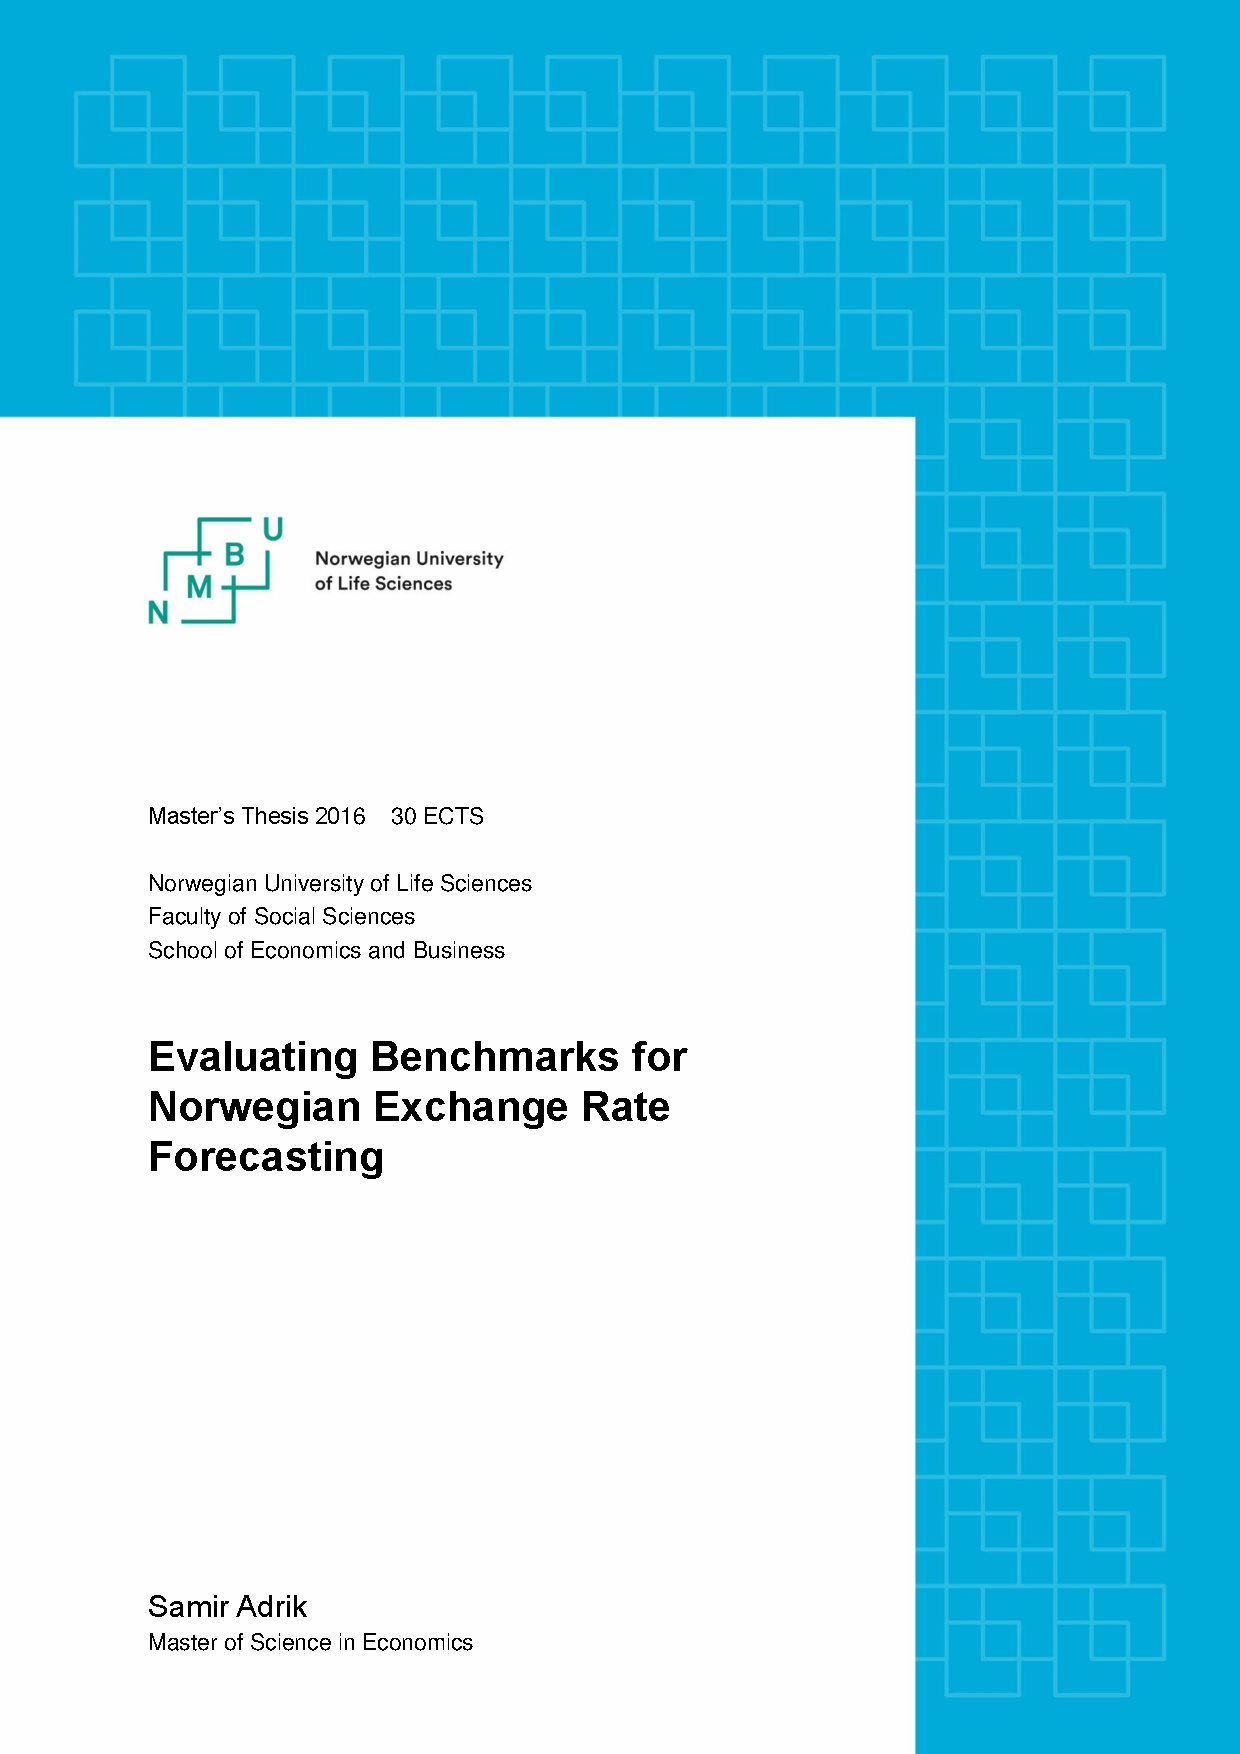
\includepdf[width=1.5\textwidth,height=1.45\textheight]{m_eng_a4.pdf}
\blankpage
\newpage
\small
\newpage
\afterpage{\blankpage}
\newpage
\begin{titlepage}
\begin{center}
\vspace*{0,8cm}\LARGE{\textbf{Evaluating Benchmarks for Norwegian\\ Exchange Rate Forecasting}}\\[0,4cm]

\vspace*{1,5cm}\Large{\textbf{Samir Adrik}}

\vspace*{3cm}
\includegraphics[scale=1.5]{images/NMBU.eps}

\vspace{1cm}\large{\textbf{Thesis submitted for the degree of\\ \textit{Master of Science in Economics}}}\\[0,5cm]

\large{\textbf{School of Economics and Business,\\
Norwegian University of Life Sciences}}\\[0,5cm]

\large{\textbf{May 18, 2016}}
\end{center}
\end{titlepage}

\newpage
\pagenumbering{roman}

\afterpage{\blankpage}
\newpage
\begin{spacing}{1.5}
\section*{Acknowledgements}

\noindent Firstly, I would like to thank my supervisor, Professor Sjur Westgaard, for helpful guidance throughout the process of writing my thesis. He has always been available to answer my questions and his many comments and suggestions have certainly been of great help.\\

\noindent I would also like to thank my family for the support and patience which they have shown over the years. They have laid a sound base for me when it comes to working with this thesis.\\

\noindent Lastly, I would like to thank all my friends from the university for making studying for this degree a memorable experience. All our debates and discussions on economic theory will surely be missed.\\

\noindent All errors or ambiguities are solely my responsibility.\\

\noindent Samir Adrik\\
Ås, May 18. 2016


\newpage
\afterpage{\blankpage}
\newpage

\vspace*{0,1\textheight}
\begin{center}
\section*{Abstract}
\end{center}

\noindent In this thesis, we compare the out-of-sample forecasting abilities of three fundamental exchange rate models (EqCM) against the random walk (without drift), RW. The objective of the thesis is to see how well the RW model performs against fundamental exchange rate models that in the literature have proven to be better at forecasting the Norwegian exchange rate. These models were tested on an out-of-sample period (2009:1-2015:4) that include two characteristic exchange rate regimes. The models estimated are well specified, but as we have found, this does not enhance the forecasting abilities.\\
\indent We find that the RW model is the benchmark of choice for Norwegian exchange rate forecasting. That is, the overall performance of the RW model is significantly better than two out of the three models tested over short-run horizons (1-4 quarters), and better than all the models over long-run horizons (16 and 28 quarters). These results are present even as we use a naive static 1-step ahead forecasting procedure. In the short run, oil prices are found to be a significant determinant for the exchange rate. In the long-run, exchange rates reflects the ratio between domestic and foreign prices. Which is in accordance with the PPP hypothesis. 
    


\newpage
\afterpage{\blankpage}
\newpage
\tableofcontents

\newpage
\pagenumbering{arabic}
\section{Introduction}
\label{sec:intro}

\noindent As an influential economic asset, the foreign exchange rate is important for many countries and institutions. It serves as a parameter for many decisions regarding foreign trade activities and the labour market. Having an idea of the factors that may cause fluctuations in the exchange rate is both important and relevant for many decision makers. Governmental institutions in particular need to understand the dynamics of the exchange rate market in order to determine appropriate monetary and fiscal policies. The initiation of these policies have both direct and indirect effects on the whole economy, and using forecasts of the exchange rate as input for policy determination is necessary. For firms trading on the international markets, movements in the exchange rate can be especially important. Large changes in the exchange rate may alter the demand structure from abroad. Meaning that the firms need to plan ahead by hedging exchange rate movements or increase market presence in domestic markets in order to maintain growth and stay competitive. The use of exchange rate forecasts may facilitate in this planning and help firms achieve these business goals. \\
\indent However, the foreign exchange market is highly volatile, and much of the trading is done at marginal levels. This makes for very difficult circumstances when trying to model exchange rates. Some have even characterized the exchange rate as arguably being the most difficult macroeconomic variable to model empirically, see e.g. \cite{amano1998exchange}. Still, much research has been done into the subject, and an often cited explanatory factor for exchange rate fluctuations includes commodity prices, and in particular the price of oil. Large changes in the price of oil is argued to be a contributing factor for among others, economic recession, trade deficits and declines in the stock market, see e.g. \cite{hamilton1983oil, hamilton2005oil}, \cite{mork1989oil}, \cite{sadorsky1999oil}, \cite{backus2000oil}, \cite{barsky2004oil} and \cite{kilian2009impact}. At the time of writing this thesis, the price of crude oil has dropped by more than 60 \% over the last year and a half\footnote{Period: July, 2014 - May, 2016.}. Similar declines have not been witnessed since the financial crisis (2007-2008), and the effects that this may have on the economy is a subject of much debate.\\
\indent Theoretically, it is argued that countries whose trade policies are highly dependent on oil may experience exchange rate appreciation when oil prices rise, and depreciation when they fall, see e.g. \cite{krugman1980oil,krugman1983oil}, \cite{golub1983oil} and \cite{corden1984booming}. The empirical literature is, however, mixed in supporting this assumed relation. For a relatively small, open and commodity based economy like Norway, empirical studies offer mixed support for this relation. As remarked by \cite{akram2000does, akram2004oil}, Norwegian evidence seem to show a negative relation as expected from the theory, but contrary to the theory allowing for non-linear relationships leads to more econometrically well specified and interpretable exchange rate models with strong predictive properties. He points out that allowing for such effects serves as encouragement against previous studies that have been pessimistic against deriving exchange rate models, with or without non-linear effects of macroeconomic variables, see e.g. \cite{meese1983out,meese1983empirical}, \cite{meese1990currency}, \cite{meese1990nonlinear, meese1991empirical}, \cite{diebold1990nonparametric} and \cite{frenkel1995empirical}.\\
\indent The reference to these studies emphasize the broad debate that has existed for more than three decades on which type of exchange rate models should be used as benchmarks for exchange rate forecasting. Historically, the initial exchange rate models were based on the behaviour of monetary macroeconomic fundamentals. These models assume that the exchange rate is a function of variables such as money supply, short-run interest rates, income and price levels, see e.g. \cite{hicks1967monetary}, \cite{dornbusch1976expectations}, \cite{frenkel1976monetary}, \cite{mussa1976exchange} and \cite{bilson1978monetary}. However, the findings of \cite{meese1983out,meese1983empirical} in particular suggest that macroeconomic effects have little influence on forecasting exchange rates. They argue among others, that the best explanatory factor to forecast exchange rates is the exchange rate itself \citep{Retief2015}. This argument is backed by their findings, which show that a simple and naive random walk (RW) model consistently performs just as well as the monetary fundamental class models over multiple forecast periods. As noted by \cite{engel1994can}, \cite{isard1995exchange} and \cite{evans2005meese}, the contributions of \cite{meese1983out,meese1983empirical} led to the identification of the RW model as a benchmark to test against for exchange rate models that lack theoretical support. This argument on the behaviour of exchange rates can be traced back to \cite{bachelier1900theory}, who is unarguably a major pioneer of modern day mathematical finance, and who proposed that financial assets are unpredictable as they follow a random walk. Early work done by \cite{reinton1999out} suggest that this argument is limited in Norway, as multivariate models can be structured to outperform the RW model. The use of RW models as benchmarks for exchange rate forecasting is also addressed by \cite{akram2000does,akram2004oil}. He finds that the non-linear fundamental exchange rate model mentioned previously outperforms the RW model, with and without drift in out-of-sample forecasting. Resent research also seem to confirm the notion that RW models are insufficient benchmarks for exchange rate forecasting, see e.g. \cite{wu2001real}, \cite{alvarez2007if}, \cite{bissoondeeal2009monetary} and \cite{Retief2015}. In Norway, additional research done by \cite{bjornland2006importance} also suggest that the choice of macroeconomic fundamentals is important, as neglecting to include interest rates in the long run, tips the scale in favour of the RW models.

\subsection{Problem Statement}
The use of RW models as universal accepted benchmarks for Norwegian exchange rate forecasting, is one we try to explore to its full potential. In this thesis we investigate: How well does the RW model (without drift) perform against fundamental exchange rate models that in the literature have proven to be better at forecasting the Norwegian exchange rate? Furthermore, given the situation in the crude oil market at the time of writing this thesis. We re-examine the role that oil price effects may play when choosing appropriate exchange rate benchmarks for the Norwegian exchange rate. To answer these questions, we analyse the statistical properties and compare the forecasting abilities of the RW model against multivariate fundamental exchange rate models over several forecasting periods. These are derived on quarterly data over the period 1988:1-2008:4, with the period 2009:1-2015:4 serving as the out-of-sample period.

\subsection{Structure}
This thesis proceeds as follows: The next section (2) presents a thorough review of the exchange rate literature to put the proposed research in a relevant context. Critics to the literature are also discussed. Section 3 details the data used and reviews the quality. Descriptive statistics are presented and limitations to the data are dealt with accordingly in this section. Section 4 presents the methodology used in order to access the forecasting performance. A discussion of the econometric models used in the literature and the differences among them are also presented in this section. The results are presented in section 5, with conclusive remarks and discussion found in section 6. Additional reading and relevant econometric output is found in the appendix.

\section{Literature Review}
\label{sec:lit}

\noindent The early exchange rate models stressed that exchange rates fluctuations should reflect movements in countries relative money, price levels, output and interest rates, see \cite{hicks1967monetary}. The intuition being that as circumstances become more favorable in the foreign market. This may stimulate capital movements out of the domestic market and thus depreciated the local currency, and vise-versa if conditions become favorable in the domestic market. By building on a small open economy model where real money is a function of output and interest rates, \cite{frenkel1976monetary}, \cite{mussa1976exchange} and \cite{bilson1978monetary} use purchasing power parity (PPP) and uncovered interest rate parity (UIRP) conditions\footnote{see appendix \ref{app:1} for further information} to obtain a relationship between exchange rates, money and output. Assume we have two countries, denoted "home" and "foreign". The asterisk (*) symbolizes the parameter of the foreign economy. Let $m_t$ be the logarithm of the money supply, $p_t$ the logarithm of the price level, and $y_t$ the logarithm of output. The real demand for money in the home country can then be modeled as, $m_t - p_t = \gamma y_t - \delta i_t$, where $\gamma$ is the elasticity with respect to income, and $\delta$ is the semielasticity with respect to interest rates. The elasticity parameters and the real demand for money is assumed to be the same in the  foreign country, i.e. $m_t^* - p_t^* = \gamma y_t^* - \delta i_t^*$. Combining both demand equations with the PPP condition, i.e. $e_t = p_t - p_t^*$, and solving for the exchange rate, $e_t$. We get the following flexible price version of the monetary model, also called the Frenkel-Musa-Bilson model. 
\begin{align}
    e_t = \delta \left(i_t - i_t^* \right) - \gamma \left(y_t - y_t^* \right) + \eta \left(m_t - m_t^*\right) + \epsilon_t
    \label{eq:1}
\end{align} 
\noindent where $\eta = 1$. In equation (\ref{eq:1}), the PPP holds at both short and long-run horizons. Prices are assumed to be flexible, e.i. that prices adjust quickly to changing market conditions. This assumption is in some ways limited as many firms hesitate to change their prices for fear that competitors will not follow suit, see \cite{blinder1994sticky} on the treatment of sticky prices in the real world. Allowing for sticky price adjustments typically implies that relative prices or inflation differentials enters into (\ref{eq:1}) directly as an independent variable. 
\begin{align}
    e_t = \beta\left(p_t - p_t^* \right) + \delta \left(i_t - i_t^* \right) - \gamma \left(y_t - y_t^* \right) + \eta \left(m_t - m_t^* \right) + \epsilon_t
    \label{eq:2}
\end{align}
\noindent Equation (\ref{eq:2}) is the sticky price version of the monetary model, also called the Dornbusch-Frankel model, see \cite{dornbusch1976expectations}. Allowing for price stickiness implies that PPP holds in the long-run, but not in the short-run. An assumption that has limited this equation, is the observed correlation between changes in the long-run exchange rate with unanticipated shocks to the current account balance. The sticky price version has thus also been extended by \cite{hooper1982fluctuations} to incorporate the effects of the current account ("the Hooper-Morton model").
\begin{align}
    e_t = \beta\left(p_t - p_t^* \right) + \delta \left(i_t - i_t^* \right) - \gamma \left(y_t - y_t^* \right) + \eta \left(m_t - m_t^* \right) + \zeta_1\bar{TB} + \zeta_2\bar{TB}^* + \epsilon_t
    \label{eq:3}
\end{align}
\noindent where $\bar{TB}$ and $\bar{TB}^*$ represent the cumulative trade balance for the home and foreign countries. The use of various forms of eqs. (\ref{eq:1}-\ref{eq:3}) to forecast exchange rates has been at the heart of the debate on exchange rate predictability with macroeconomic fundamentals. Empirically, these models may be generalised to include $n$ relative and $m$ additional fundamental variables, i.e.
\begin{align}
e_t = \sum_{i=1}^n\alpha_i(f_{i,t}-f_{i,t}^* )+\sum_{j=1}^m\alpha_j (F_{j,t}+F_{j,t}^*)+\epsilon_t \hspace{0,5cm}\text{where}\hspace{0,5cm} i\neq j
\end{align}
Focusing on the out-of-sample forecasting abilities, \cite{meese1983out,meese1983empirical} finds that the random walk model without drift, i.e  $e_{t} = \rho_1 e_{t-1} + u_t$, where $\rho_1 = 1$ and $u_t$ is iid with $\left(0,\sigma^2 \right)$, forecasts exchange rates equally well as (\ref{eq:1}-\ref{eq:3}), and in some cases even better. This empirical irregularity has come to be known as "the Meese and Rogoff puzzle". The findings have over the last three decades been confirmed by multiple authors using various time horizons and additional explanatory factors, e.g. differences in productivity. \cite{cheung2005empirical} express relative prices $\beta\left(p_t - p_t^* \right)$ as a function of productivity differences $z_t$, which is in line with theory presented by among others, \cite{balassa1964purchasing} and \cite{samuelson1964theoretical} ("the Balassa-Samuelson effect"). They find that models that add productivity differentials do not forecast exchange rates better than the random walk. Further research done over short horizons (less than one year) and long horizons (one to five years) have all come to confirm the identification of the RW model (without drift) as the toughest benchmark for forecasting exchange rates see e.g. \cite{chinn1995banking}, \cite{alquist2008conventional} and \cite{molodtsova2009out}.\\
\indent However, this argument is equally dismissed by many, suggesting that the debate is still alive and well. Recent international research have come to argue that the RW models are actually insufficient benchmarks for exchange rate forecasting, see e.g. \cite{wu2001real}, \cite{alvarez2007if}, \cite{bissoondeeal2009monetary} and \cite{Retief2015}. Norwegian evidence also seem to offer support to this conclusion, as research suggests that there may be some scope for the monetary models in forecasting the Norwegian exchange rate. This is not simply by the use of eqs. (\ref{eq:1}-\ref{eq:3}), but focusing attention on commodity prices as a potential new macroeconomic fundamental. The term "commodity currency" is one that is almost synonyms with the Norwegian exchange rate, as oil and gas accounts for almost 50 \% of the total exports in Norway\footnote{see e.g. \cite{SSB1} and \cite{bjornland2013} who finds that 30-40 \% of the variation in economic growth in the Norwegian mainland is linked to oil.}. \cite{reinton1999out} found early on evidence that a single equation monetary model outperforms the RW model in out-of-sample forecasting exercises for Norwegian data. Their findings suggested that the outperformance was only witnessed over relative short 6 and 12 months horizons, and this without including the oil price as an explanatory factor. Still, their findings did show that the RW model has its limitation on Norwegian data. This addition has come to be an interesting point in recent years. \cite{akram2000does, akram2004oil} found that by structuring models so that they allow for non-linear oil price effect makes for even better forecasts of the Norwegian exchange rate. By following this framework, one improves the forecasts compared to simple linear models and the toughest benchmark, namely the RW model substantially. This outperformance was witnessed over 12 quarters, and thus suggests that the non-linear oil price effects are of importance in the long-run. Recently, \cite{papadamou2012monetary} and \cite{papadimitriou2014forecasting}, re-tested many of the fundamental monetary models as mentioned previously on Norwegian data, and they provide empirical in-sample evidence for proportionality between the exchange rate and many of the fundamental determinants in Norway. However, they do not compare the forecasting abilities of the fundamental models against the RW model in out-of-sample forecasting competitions. Their findings are not only limited to Norway, as similar findings from other international currencies may suggest that the monetary models are still relevant and on the international agenda, see e.g. \cite{chin2007monetaryb, chin2007monetary}, \cite{tawadros2008structural} and \cite{loria2010new}. In general, \cite{chen2003commodity} also confirms that there is empirical in-sample evidence in favour of commodity prices as predictors for the exchange rate. However, \cite{chen2010predicting} finds that commodity prices are not good out-of-sample predictors. Which shows that there is still no uniform agreement to the use of commodity prices in forecasting exchange rates. Additionally, \cite{bjornland2006importance} find that oil prices are not necessarily the most important factor for beating the RW in Norway. Their focus is on interest rates, and they conclude that by ignoring the interest rate differential in the long-run, a structural fundamental model would not beat the RW model in out-of-sample forecasting competitions. The model used by \cite{bjornland2006importance} preforms just as well as the RW model over long horizons, but consistently outperforms the RW over short horizons (less than 1 year).\\
\indent To recap the literature review, we can say the following: To forecast exchange rate has been an integral part of empirical financial economics since the 1960s. Two different arguments have been proposed in the debate on the ability to forecast exchange rates, and whether it is even possible. The first states that macroeconomic information is a continuously important component for building exchange rate models with predictive power, and routed in economic theory. The second (which goes against the first) is that the models proposed thus fare are too simplistic and have little to no predictive power compared to the RW model. This implies that macroeconomic information is no needed as a prerequisite. Norwegian research by among others, \cite{reinton1999out}, \cite{akram2000does,akram2004oil} and \cite{bjornland2006importance} all provide evidence against the second and seems to suggest that Norway is a country that is in a somewhat special position, and one that may not be representative for "the Meese and Rogoff puzzle". This thesis will humbly try to offer a contribution to the mentioned debate by investigating models in the recent literature (see section \ref{sec:meth}) that all claim to beat the RW over varying time horizons. More specifically, the following can be said to be the contributions of this thesis: (1) The extensive use of equilibrium correction (error correction) models, EqCM that have been successful at varying time horizons may offer a narrowing of the search area for the appropriate specifications of fundamental exchange rate models on Norwegian data. (2) The testing of these models may provide further insight into how EqCM perform under varying exchange rate regimes. (3) As oil is an important resource for Norway, the inclusion of oil price effects in the models tested may offer additional insights into the importance of commodity prices as a fundamental exchange rate determinate.\\
\indent We need to emphasize that the models used in this thesis only include non-panel data estimation methods. According to \cite{engel2007exchange}, it is this over-reliance on non-panel data modelling techniques that makes beating the RW model difficult. They provide evidence that with the use of panel data techniques, monetary models can be estimated so that they beat the RW model in out-of-sample forecasting competitions. They also highlight and offer warnings that out-of-sample forecasting power relative to the RW is an unreliable gauge for evaluating exchange rate models, as exchange rates are asset prices driven by expectations. The fact that we don't have a direct way of measuring market expectations, implies a limitation for exchange rate models as they cannot be tested directly.


\section{Data}
\label{sec:data}

\noindent In this section we present the data used in this thesis. The first step is to determine the variables that are of interest. Following among others, \cite{reinton1999out}, \cite{chin2007monetary,chin2007monetaryb} and \cite{papadamou2012monetary}, the most important point to the models tested in this thesis, is to take into account the differences in the macroeconomic fundamentals between Norway and the foreign market. In this thesis, the foreign market constitute the historically largest 15 trading partners of Norway, namely Belgium, Canada, China, Denmark, Finland, France, Italy, Japan, the Netherlands, Poland, Spain, Sweden, the United Kingdom and the United States. The mentioned countries have collectively accounted for more than 80 \% of the total trade with Norway since the late 1980s. This serves as the main motivation for having them represent the foreign market. The sample period consists of quarterly observations from 1988:1 - 2015:4. We reserve the last 28 quarters (2009:1-2015:4) as the out-of-sample period. The reason being that this period is characterized by two main exchange rate regimes. During the first 16 quarters (2009:1-2012:4), the Norwegian krone exhibited a strong appreciation (-11 \%), with the final 12 quarters (2013:1-2015:4) showing the opposite (depreciation of 25 \%). The changing exchange rate regimes provides us with strong circumstances for testing the role that fundamental determinants play in explaining alternating exchange rate regimes. Furthermore, we choose to split the out-of-sample period into several forecasting period, all of whom are common in the literature (see section \ref{sec:meth}). Rather than model a single bilateral Norwegian exchange rate pair (e.g. NOK/EUR or NOK/USD), we follow \cite{akram2000does,akram2004oil}, and try to model changes in the trade weighted index (TWI) of NOK as presented by \cite{NBa}. The TWI is a nominal effective exchange rate index of the Norwegian kroner calculated against the currencies of the 25 main trading partners of Norway. The index is a geometric average using weights from the OECD, and the calculation of the index is based on the product of a chain of Laspeyres’ index formula. 
\begin{align}
    E_t = \prod_{i=0}^N\left(\frac{S_{i,1}}{S_{i,0}} \right)^{w_{i,0}}\prod_{i=0}^N\left(\frac{S_{i,2}}{S_{i,1}} \right)^{w_{i,1}}\hdots \prod_{i=0}^N\left(\frac{S_{i,T}}{S_{i,T-1}} \right)^{w_{i,T-1}}  
\end{align}
\noindent where $S_{i,0}$ is the base level of exchange rate (nominal) $i$, $S_{i,t}$ is the exchange rate $i$ at time $t$, $w_{i,0}$ is exchange rate $i$'s weight in the base year, $N = 25$ and $t=0,\hdots,T-1, T$. The value of the index over a period is split into small periods, and each product operator $\prod$ typical represents a one year period. The intuition for choosing to model an exchange rate index rather than a single exchange rate pair, is due to the broader capturing of movements in the Norwegian exchange rate. In this thesis, we employ seasonally unadjusted quarterly data. This is to ensure that differences in seasonal adjustments among the independent variables don't effect the overall estimation, or add additional information that may distort the estimation. To correct for seasonality, we follow \cite{reinton1999out} and use quarterly dummy variables as additional independent variables. Impulse dummies are also added to address outliers. The determinations of these are based on a general-to-specify method in order to assure normality of residuals and additional diagnostics. All the variables will be in percentage term, and thus unit free. The price levels used are represented by the consumer price index (CPI) in Norway and a trade weighted average of consumer price indeces of Norway's trading partners. According to the empirical research, different proxies are typically used for the unobserved expected inflation rate\footnote{see e.g. \cite{reinton1999out} and \cite{papadamou2012monetary} for estimations with different inflation expectation proxies.}. We choose not to proceed with this scheme due to limtiations. We follow \cite{akram2000does,akram2004oil} and only include differences in CPI inflation between Norway and its trading partners. Unlike \cite{meese1983out,meese1983empirical}, we use M3 as the measure of broad aggregate money supply. The M3 measure is also given by a trade weighted average index for the main trading partners mentioned above, and we use M3 as it is the broadest measure of money supply used by among others the OECD. The price of oil is given by the Brent Blend crude price, but following \cite{bjornland2005commodity} and \cite{papadamou2012monetary} it is theoretically possible that the oil price may cause the exchange rate to diverge from the PPP. To counter for this, the real oil price is added to the models tested. The interest rate variables used in this thesis include both short- and long-run interest rates. As short-run interest rates, we use three months money market rates. The long-run interest rates are given by the returns on government bond with 10 years maturity. Measure of output/real income is given by indices for industrial production. As mentioned by \cite{reinton1999out}, the accuracy of industrial production as proxies for real income may change and differ over time as the economic development of countries change. Rather than looking at the variables independently, we always follow theory and try to structure the variables so that they reflect relative differences between Norway and the foreign market. All the variables, the direct sources and some of the transformations can be found in Table (\ref{tab:var}). The descriptive statistics for both the in sample and out-of-sample periods can be found in Tables (\ref{tab:desc})-(\ref{tab:descouts}). Figure (\ref{fig:tspvar}) also shows a time series plot of the quarterly observations of selected variables over the full sample period (1988:1-2015:4). Accoring to the literature additional variables may be included to the fundamental models, e.g. Taylor rule fundamentals, portfolio balance etc. But due to limitations, these will not be included in the thesis. We recommend \cite{rogoff2008continuing} and \cite{rossi2013exchange} for an overview of the variables that are used in the literature and the forecasting performance of these. All the calculations in this thesis are done with the use of the econometric software Gretl \citep{gretl} and PcGive 14.0 \citep{doornik1997pcgive}. \\
\indent As the data used in this thesis is time-series, we conduct tests to insure that the quality of the data is in line with the underlying assumptions following the estimation methods used for the different models presented in the later chapter. Firstly, Table (\ref{tab:adf}) shows the Augmented Dickey-Fuller (ADF) test for stationarity \citep{dickey1979distribution} for the log and first difference form of the mentioned variables used in this thesis. As expected from econometric theory, we can conclude that the level forms of the variables exhibit evidence against stationarity for almost all variables\footnote{Dickey-Fuller tests cannot reject the presence of unit root in all series, except $cpi-cpi^*$, $i_s - i_s^*$ and $FI.Y$ which are found to be I(0) at 5\%.}. By structuring the variables with the first difference, the variables become stationary. This means that the variables are integrated in first order I(1) and their variances are finite. We also know from econometric theory that the use of variables in first difference form may lead to loss of long-run information about any potential models. Therefore, tests for cointegration are necessary to check for the presence of any possible long-run relationship among the variables. As the variables may exhibit cointegration, we conduct two separate tests for this. In order to avoid pitfalls for testing for long-run relationships, we follow the recommendations of \cite{gonzalo1998pitfalls} and apply the \cite{engle1987co} two-step procedure and the \cite{johansen1991estimation} test for cointegration\footnote{The \cite{johansen1991estimation} test takes into consideration the number of cointegrating vectors in the null hypothesis, see appendix \ref{app:2} for further information}. The null hypothesis for both tests is that there exists no cointegration vector, i.e. that no combinations of I(1) variables move together through time, and that follow a long-run equilibrium relation. By rejecting the null hypothesis of no cointegration vector this implies that a long-run relationship exists between the variables. Table (\ref{tab:coint}) presents the results of the cointegration test. From the results, we can see that the \cite{engle1987co} test suggests that there are no cointegrating vectors as the null can't be rejected for both the test structure that includes a trend and the one that does not. To this we need to emphasize that the \cite{engle1987co} test has its limitations, and one is that it can only identify one single cointegrating relation among many in a variable set. The \cite{johansen1991estimation} test addresses this issue as it allows for identifying multiple cointegrating relations. The test results presented in Table (\ref{tab:coint}) include both the trace and maximum eigenvalue ($\lambda$-max) approach. Both test statistics seem to provide evidence against the null hypothesis of no cointegration. Using the trace test, we can reject the null hypothesis $r=2$ at conventional significance levels. But by using the $\lambda$-max approach the results differ, and its only at $r=1$ we can reject the null. A common problem with the \cite{johansen1991estimation} test is that for small sample sizes ($N < 100$) the results may not be reliable as it alone does not serve as a good approximation for variables of finite sample, see e.g. \cite{cheung1993finite}, \cite{gonzalo2000robustness}, \cite{silvapulle2000effect} and \cite{hubrich2001review}. To counter for this, we also conduct a third trace test that adjusts for the sample size, see \cite{johansen2002small}. The results seem to be in-line with the results from the $\lambda$-max test. At 1 \% significance both the $\lambda$-max and the adjusted trace test cannot reject the null of two cointegrating vectors $r=2$. Hence, there is strong evidence of at least one cointegrating relationship in the system. Similar results are reported by \cite{bjornland2006importance} and \cite{papadamou2012monetary}.       
 
\section{Methodology}
\label{sec:meth}
 
\noindent As the results from the previous section suggest that there is presence of cointegration by means that we cannot reject the null hypothesis of no cointegration vector for $r=2$. This implies that a long-run relationship among the variables exists. The next step would be to establish this long-run relationship. The empirical research have come to structure models with different intuition for the establishment of this relationship. This suggests that the there is no uniform consensus for the correct treatment of the observed cointegration relation as presented in the previous section. According to the Engle-Granger representation theorem (EGRT) \citep{engle1987co}, if a cointegration relationship between I(1) variables exists, then an equilibrium correction (error correction) model, EqCM can be applied to show the influence of the long-run relationship on the short-run dynamics of the variables tested in the model. In addition, in an EqCM model, short- and long-run effects on exchange rates can be investigated both independently and collectively. The use of the EqCM framework is widely used in the literature, and thus serves as motivation for including this framework as a natural part of the thesis. The EGRT also states that systems with cointegrated I(1) variables, in addition to EqCM, have equivalent representation with common trends (CT) and moving averages (MA) models. In this thesis, we will not address any of these frameworks, but recommend e.g. \cite{baillie1989common}, \cite{crowder1994foreign}, \cite{enders1994theory}, \cite{sarno2002economics} and \cite{mizuno2006modeling} for further information about the applications of CT and MA models on exchange rates.\\
\indent In this thesis, we'll be testing three separate, but similar EqCMs used in the literature. All have shown to be effective at outperforming the RW model on Norwegian data at different time horizons. The first possible EqCM is based on \cite{reinton1999out}, and builds on eqs. (\ref{eq:1}) and (\ref{eq:2}), where the long-run proportionality is describes by an error correction term between the exchange rate and the relative money supply. Following the sticky price criticism of the Frenkel-Musa-Bilson model (\ref{eq:1}), an assumption of non-instantaneous adjustment of the actual exchange rate to its equilibrium value is made by introducing the lagged dependant variable of the exchange rate, $e_{t-1}$ in the model. As we will see, this is not an uncommon assumption as both lagged values and differences of both the dependant and independent variables is often used in the literature. By allowing for this specification one can access a wider variety of dynamic patterns in the data.  The econometric methodology used for almost all models is a general-to-specific approach \citep{krolzig2001computer}. After testing all the models for misspecification, we simplify the models by removing variables that are statistically insignificant. This is done for the sake parsimony, i.e. explaining changes in the exchange rate using few parameters\footnote{The second model (\ref{eq:ecm2}) does not follow this approach as we seek parsimony by re-investigating the findings of \cite{bjornland2006importance} with an almost similar functional specification.}. The first error correction specification is given by the following.   
\begin{align}
    \Delta e_t = \mu + \sum_{j=1}^m \beta_j \Delta (f_{j,t}-f_{j,t}^*) + \sum_{i=1}^k \eta_{i} \left(e - m + m^* \right)_{t-i} + \sum_{j=1}^p \omega_j e_{t-j} + \phi \mathbf{D}_t + \epsilon_t
    \label{eq:ecm1}
\end{align}
where $\Delta$ denotes the change from the previous period, lag order $k = p = 1$ and the fundamental relative macroeconomic variables $f$ and $f^*$ are structured in accordance with eqs. (\ref{eq:1}) and (\ref{eq:2}). The parameter $\eta$ represents the effects of a long-run equilibrium relation to changes in the exchange rate ($\Delta e_t$). Following \cite{reinton1999out}, we need to emphasize a particular point about this proposed long-run relationship. Money supply is not known with certainty at any given time. As these variables are typically published with a lag or with a contingency of future revision. We assume that although the series are subject to uncertainty, the model can make actual exchange rate forecasts using the available economic data. $\mathbf{D}_t$ contains all the deterministic components such as time trend, seasonal and impulse dummies. Also note that the impulse dummies are chosen based on an outlier procedure\footnote{Influential observation function based on influence and leverage points, Gretl (PcGive can also be used).}. Furthermore, we will only use the Dornbusch-Frankel specifications, i.e. the price differential will always enter into the models, either relatively or independently.\\
\indent The parsimoniously representation of (\ref{eq:ecm1}) is presented in Table (\ref{tab:ecmtab1}). As we can see, the error correction term is positive and very significant. This suggests that the error correction term works to induce a positive change in the exchange rate back to its long-run equilibrium. Indicating that a long-run proportionality between exchange rate and money supply may exist, but contributions to the forecasting may be limited as the exchange rate adjusts in the wrong direction. This is contrary to the findings of \cite{reinton1999out}, who finds positive, but insignificant long-run specification for half of the spot rates examined their article. This irregularity may be due to us modeling changes in the TWI and not bilateral exchange rate pairs. The short-run effects as represented by changes in the relative money supply between Norway and the foreign market shows to be negative and significant. This means that money supply has appreciation pressure on the Norwegian exchange rate, and is in accordance with the theory. The functional form seems to be adequate as tests for misspecification cannot reject the null. We need to emphasize that although the RESET test is clear on adequate specification, the non-linearity test \citep{saikkonen1988lagrange} is almost rejected at 5\%, suggesting that the money supply effects may be non-linear. By means of the outlier procedure, we detect four clear outliers that are picked up by impulse dummies in the model: $id97q1$, $id02q2$, $id08q2$ and $id08q4$. All represent different stages of the Norwegian exchange rate history, and include periods of strong appreciation and depreciation pressure that may be caused by turmoil in international equity markets. The use of these dummies are widely reported in the literature, and will also be used in the later models. Given a relatively small number of regressors ($k = 8$), the adjusted goodness-to-fit is 45\% with a log-likelihood of 234. All the underlying assumptions of the estimation are fulfilled at conventional levels of significance (see the diagnostics in Table \ref{tab:ecmtab1}). By not including the impulse dummies this would not be the case, as it would cause problems with normality of residual terms, heteroscedasticity and autoregressive conditional heteroscedasticity, ARCH effects.\\
\indent The second possible EqCM is based on research done by \cite{bjornland2006importance}. It combines the PPP condition with the interest rate differential to form the long-run equilibrium relation. They provide evidence that a pure PPP model would not suffice to beat the RW, but by combining PPP and the interest rate differential allows for stronger forecasting power. The EqCM is given by the following specification:
\begin{align}
\nonumber    \Delta e_t = \mu &+ \sum_{j=1}^{p-1} \gamma_{1j} \Delta e_{t-j} + \sum_{j=0}^{p-1} \gamma_{2j} \Delta p_{t-j} + \sum_{j=0}^{p-1} \gamma_{3j} \Delta p^*_{t-j} + \sum_{j=0}^{p-1} \gamma_{4j} \Delta i_{t-j} + \sum_{j=0}^{p-1} \gamma_{5j} \Delta i_{t-j}^*\\
    &+ \sum_{i=1}^k\rho_i\left(e - p + p^* \right)_{t-i} + \sum_{i=1}^k \omega_{i}\left(i - i^* \right)_{t-i} + \phi \mathbf{D}_t + \epsilon_t
    \label{eq:ecm2}
\end{align}
where the lag order $p=4$, and the error correction term is described by a split of two parts: The pure PPP and the interst rate differential\footnote{The fact that we include two equilibrium (error) correction terms, means that the models becomes a vector equilibrium (error) correction model, VEqCM.}. Accordingly, the term $(e - p + p^*)_{t-k}$ and possibly the constant term $\mu$ represent a deviation from the equilibrium level under the PPP hypothesis. The interest rate differential $(i-i^*)_{t-k}$ represents a proxy for possible appreciation to the exchange rate according to the uncovered interest rate parity (UIRP) hypothesis. The error correction terms are lagged by one period, i.e. $k=1$. We can also see from the model that lags of the exchange rate, prices and interest rates are inputted as unrestricted variables. This is due to an assumption of non-symmetry and thus the mentioned variables are representative for the short-run effects in the model (which is typical of EqCM).\\
\indent The final parsimony model of (\ref{eq:ecm2}) is presented in Table (\ref{tab:ecmtab2}). From the results, we can see that the pure PPP term is negative and significant. This implies that the exchange rates will in the long-run move towards equilibrium, and has the expected sign. More specifically, the exchange rate adjusts in the right direction. The interest rate differential also seem to have the same long-run effect on the exchange rate. In the short-run, changes to the unrestricted $cpi$ terms seem to have depreciation pressure, with the $cpi^*$ terms having the opposite signs. The impulse dummies are all negative and significant for the outliers that represent strong appreciation ($id97q1$, $id02q2$, $id08q2$), with the opposite sign for the outlier of depreciation ($id08q4$). The functional form specification seems to be adequate, and even stronger than the previous EqCM (\ref{eq:ecm1}). This can be seen as the RESET and non-linearity test are more insignificant. The number of regressors is high compared to (\ref{eq:ecm1}), and accordingly we "lose" explanation power as the adjusted goodness-to-fit is 37\% (compared to 45\%). The estimated log-likelihood is at 225. All the underlying assumptions are intact as expected.\\ 
\indent The third and final EqCM is based on an augmented version of the model presented by \cite{akram2000does,akram2004oil}. This model comes in two forms. One is a linear model with symmetric oil price effects, and the second is a model with non-linear oil price effects. The latter is not considered in this thesis. However, we will run several tests to check whether the relationship is linear to investigate if a non-linear functional form of oil prices is relevant. The EqCM specification is given by: 
\begin{align}
\nonumber    \Delta e_t = \mu &+ \sum_{j=1}^{p-1} \gamma_{1j} \Delta e_{t-j} + \sum_{j=0}^{p-1} \gamma_{2j} \Delta p^*_{t-j} + \sum_{j=0}^{p-1} \gamma_{3j} \Delta i_{t-j}^* + \sum_{j=0}^{p-1} \gamma_{4j} \Delta FI.Y_{t-j} \\\nonumber
&+ \sum_{j=0}^{p-1}\gamma_{5j}\Delta \left(i_{t-j} - \Delta p_{t-1-j} \right) + \sum_{j=0}^{k}\Omega_{i}\left(e_{t-i} - \Phi roil_{t-i} \right)\\ 
&+ \sum_{i=1}^k\rho_i\left(e - p + p^* \right)_{t-i} + \phi \mathbf{D}_t + \epsilon_t
    \label{eq:ecm3}
\end{align}
where the lag order $p = 4$ and $k = 1$, which is the same as in (\ref{eq:ecm2}). The error correction term in (\ref{eq:ecm3}) is given by a long-run proportionality between the level of the exchange rate and the real oil prices. In addition, we introduce some new variables. The term $ \Delta (i - \Delta p)$ represents changes to the "real interest rate", and should be expected to place appreciation pressure on the exchange rate. According to \cite{akram2000does, akram2004oil}, including this variable is done in order to sought out parsimony by restricting changes in the domestic interest rate and the inflation rate terms to an interpretable variable of changes in the domestic real interest rate. More specific, by doing this parsimony simplification the $\Delta p$ and $\Delta i$ terms from the previous model (\ref{eq:ecm2}) become one term, thus decreasing the number of regressors. $\Delta FI.Y$ is changes to the current account, and should according to \cite{hooper1982fluctuations} have the opposite sign and thus pressure the exchange rate by depreciation.\\  
\indent The parsimoniously representation of (\ref{eq:ecm3}) is listed in Table \ref{tab:ecmtab3}. From the results, we can see that the long-run relationship between exchange rates and real oil prices seem to be present. The coefficient is negative and highly significant. This suggests that this long-run relation works to correct the exchange rate back to its long-run equilibrium. Changes to the current account also seem to have the expected signs. The number of regressors is higher than the first model, but lower than the second. Still, this induces the highest adjusted goodness-to-ft (48\%). Similar to the second EqCM (\ref{eq:ecm2}), the diagnostics tests seem to show a clear upholding of the underlying assumptions for the OLS estimation method. \cite{akram2000does,akram2004oil} finds that the linear model may be subject to misspesfication, due to the presence of possible non-linear relations of the oil price effecting the exchange rate. Based on our results, we can see that both the RESET and Squares.LM.$\chi^2$ test for functional form seems to suggest adequate specification. Now that we have determined three possible long-run relationships to counter for the problem with cointegration mentioned in section (\ref{sec:data}). We move on to test the forecasting abilities of the models presented.

\section{Empirical Results}
\label{sec:res}

\noindent In this section, we present the results of the out-of-sample forecasting competitions. We follow \cite{meese1983out,meese1983empirical} and perform the forecasting exercises with a comparison between the structural EqCM estimated in the previous section and the random walk (without drift). More specifically, the models are first estimated over the initial estimation period (1988:1-2008:4), which leaves us with a forecast period of almost 7 years. We then employ the use of a (naive) \underline{static} rolling 1-step ahead regression methodology to generate forecasts of the relative changes to the exchange rate at 1-4, 16, and 28 quarters into the future. The first forecast periods (1-4  quarters) are common in the literature, and correspond well with the duration of standard forward contracts, see e.g. \cite{meese1983out,meese1983empirical}, \cite{reinton1999out} and \cite{bjornland2006importance}. The 16 quarter horizon represents the end of the strong appreciation period that the Norwegian kroner witnessed in the first half of the out-of-sample period (see Figure \ref{fig:tspvar} and section \ref{sec:data}). The final period horizon (28 quarters) represents the whole out-of-sample period. The forecasting methodology used is very simple as it forecasts 1-step ahead based on observed observations that precede the forecasted period. As the method is very naive and simple, it may supply us with a picture of the performance of the estimated models. If the models can't outperform the RW with this naive and simple forecasting scheme, chances are small for them doing so with more complicated forecasting methodologies\footnote{In the literature, k-period rolling \underline{dynamic} methods are typically used.}.\\
\indent The literature employs various evaluation criteria for the forecasting abilities. In order to align the results of this thesis with that of the \cite{meese1983out,meese1983empirical}, we employ the use of the root mean square error (RMSE) as the principal evaluation criteria. Based on all the forecasts produced by the 1-step procedure at the different horizons, we average the squared differences to the actual realised change in exchange rate. The model with the lowest RMSE for a given horizon is defined as the superior model. A second measure that is also included is the mean absolute error (MAE), which according to \citep{meese1983out,meese1983empirical} may prove to be better than RMSE, as exchange rates may exhibit fat tails\footnote{This may be the case as the level values ($e$) have a positive excess kurtosis as can be seen in Table (\ref{tab:desc}).}. It's undeniable that the RW model is the benchmark of choice for many studies done in the literature. To address this point, we also include a direct measure of the forecasting performance against the RW model, by looking at the RMSE and MAE of the different models relative to that of the RW model. The evaluation criteria are given by the following equations:
\begin{align}
    RMSE = \sqrt{\frac{1}{n}\sum_{i=1}^n\left( \theta - \hat{\theta}\right)^2}, \hspace*{0,5cm} MAE = \frac{1}{n}\sum_{i=1}^n \left| \theta - \hat{\theta} \right|
    \label{eq:evaluate}
\end{align}
\noindent where $\theta$ is the actual change in exchange, and $\hat{\theta}$ is the estimated change. The evidence using the various criteria (\ref{eq:evaluate}) is reported in Table (\ref{tab:res}). Based on the results, it seems that almost all of the estimated models in section \ref{sec:meth} cannot claim to beat the RW in forecasting the exchange rate. Model (\ref{eq:ecm3}) is a small exception. Over the short-run (less than one year, 4 quarters) oil price effect seem to be the main driving factor for the Norwegian exchange rate. We can see this as the linear oil price effects model seem to outperform the RW model over the 1-4 horizon. The RMSE is on average 67\% lower than the RW model over the first 4 quarters, and 25\% higher in the last two horizons. The outperformance is decreasing as the horizon increases, and at 16 quarters the RW is considerably better. Over the full out-of-sample period the PPP-UIRP model (\ref{eq:ecm2}) seems to be the closest at outperforming the RW. The forecasting abilities of this model gets gradually better as the time horizon increases, suggesting that the PPP condition is an important assumptions and driving force for the Norwegian exchange rate in the long-run. This confirms the results by \cite{akram2000ppp}, \cite{akram2002ppp,akram2006ppp} and \cite{nordbo2004ppp}, who reports that the theory of PPP is very consistent with the Norwegian exchange rate in the long-run.\\
\indent The relative money supply proportionality model (\ref{eq:ecm1}) performs consistently worse at all horizons compared to the RW. The forecasts performance is clearly worse as time goes on, and this may be due to the significant long-run effect of money-supply that works to adjust the exchange rate in the wrong direction. The RMSE for this model is on average 46\% higher than the RW model over all horizons. This is contrary to the research done by \cite{reinton1999out}, but this may be due to several factors. We employ a different forecasting methodology, time frequency, smaller sample and have an out-of-sample period that is characterized by a different exchange rate regime (see Figure \ref{fig:tspvar}).  
\newpage
\newgeometry{top=2cm,bottom=2cm}
\begin{figure}[h!]
\begin{subfigure}{.5\textwidth}
  \centering
  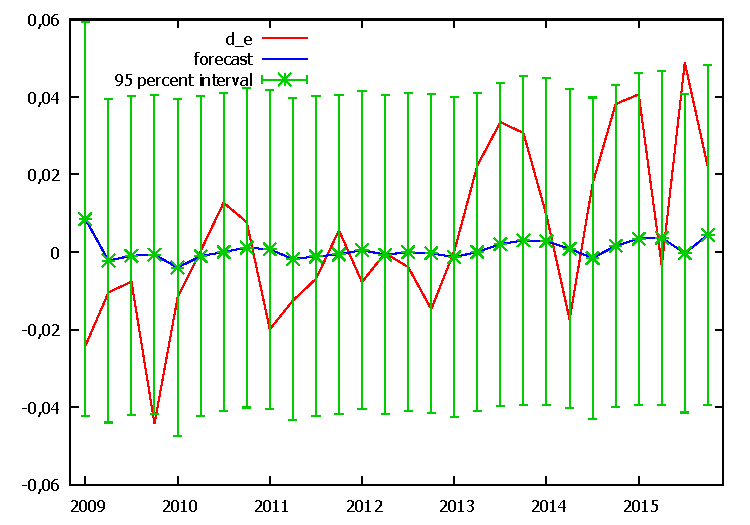
\includegraphics[width=\linewidth]{images/RWForecast.pdf}
  \label{fig:sfig1}
\end{subfigure}%
\begin{subfigure}{.5\textwidth}
  \centering
  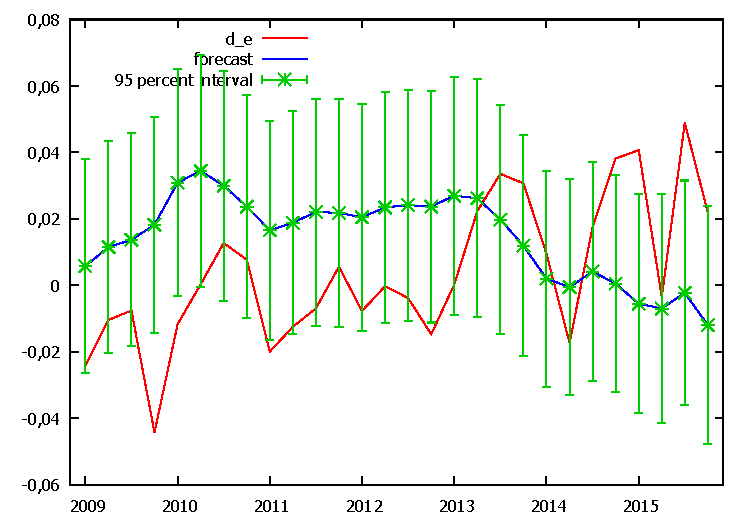
\includegraphics[width=\linewidth]{images/ReitonForecast.pdf}
  \label{fig:sfig2}
\end{subfigure}
\begin{subfigure}{.5\textwidth}
  \centering
  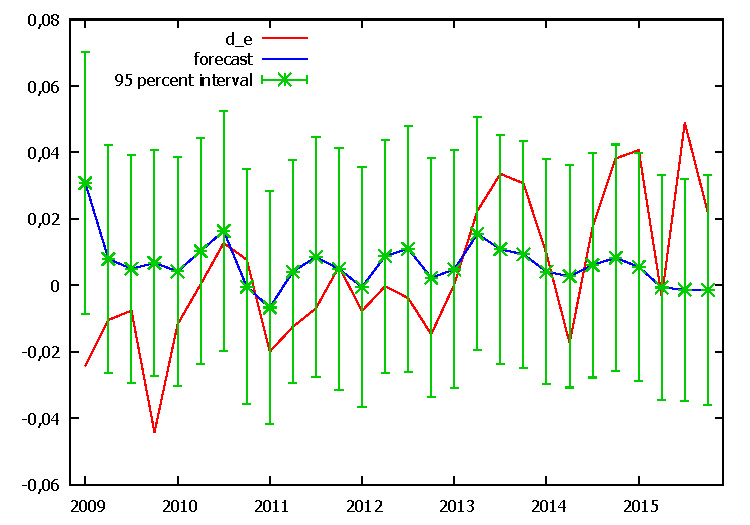
\includegraphics[width=\linewidth]{images/BjornlandForecast.pdf}
  \label{fig:sfig3}
\end{subfigure}
\begin{subfigure}{.5\textwidth}
  \centering
  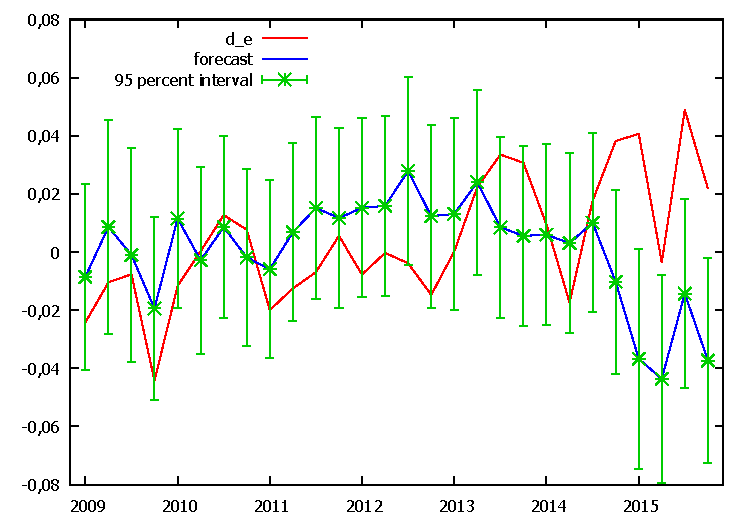
\includegraphics[width=\linewidth]{images/AkramForecast.pdf}
  \label{fig:sfig4}
\end{subfigure}
\vspace*{-0,5cm}\caption{\textit{\small Actual values (red lines) and static 1-step ahead forecasts of $\Delta e$ with 95\% prediction intervals (blue and green). Row 1: Random walk without drift (left) and relative money supply proportionality (right). Row 2: Combined PPP and UIRP (left) and linear oil price effects (right).}}
\label{fig:fig}
\end{figure}

\scriptsize
\begin{tabularx}{\textwidth}{lrrrrr}
\caption{Results from the static 1-step ahead out-of-sample forecasting exercise.}\vspace*{-0,7cm}\\
\parnoteclear\\
\toprule
\multicolumn{6}{c}{PANEL I: Root Mean Square Error (RMSE)\parnote{Note: Values in the square brackets represent measure of evaluation criteria relative to the RW (=1). Where the out-of-sample horizon is 2009:1-2015:4.}} \\
\midrule    
Period & Horizon & RW (without drift) & \multicolumn{1}{c}{EqCM (\ref{eq:ecm1})} & \multicolumn{1}{c}{EqCM (\ref{eq:ecm2})} & \multicolumn{1}{c}{EqCM (\ref{eq:ecm3})} \\
\midrule
2009:1-2009:2 & 1     & 2.617 & 2.629 [1.004] & 4.102 [1.567] & 1.745 [0.667] \\
2009:1-2009:3 & 2     & 2.168 & 2.475 [1.142] & 3.428 [1.581] & 1.476 [0.681] \\
2009:1-2009:4 & 3     & 2.866 & 3.789 [1.322] & 3.914 [1.365] & 1.784 [0.622] \\
2009:1-2010:1 & 4     & 2.578 & 3.887 [1.508] & 3.572 [1.385] & 1.905 [0.739] \\
2009:1-2012:4 & 16    & 1.663 & 3.193 [1.920] & 2.221 [1.336] & 1.863 [1.120] \\
2009:1-2015:4 & 28    & 2.126 & 3.014 [1.418] & 2.292 [1.078] & 2.982 [1.402] \\
\midrule
\multicolumn{6}{c}{PANEL II: Mean Absolute Error (MAE)} \\
\midrule
Period & Horizon & RW (without drift) & \multicolumn{1}{c}{EqCM (\ref{eq:ecm1})} & \multicolumn{1}{c}{EqCM (\ref{eq:ecm2})} & \multicolumn{1}{c}{EqCM (\ref{eq:ecm3})} \\
\midrule
2009:1-2009:2 & 1     & 2.180 & 2.597 [1.191] & 3.668 [1.683] & 1.737 [0.797] \\
2009:1-2009:3 & 2     & 1.664 & 2.443 [1.468] & 2.866 [1.722] & 1.379 [0.829] \\
2009:1-2009:4 & 3     & 2.331 & 3.394 [1.456] & 3.425 [1.469] & 1.657 [0.711] \\
2009:1-2010:1 & 4     & 1.986 & 3.567 [1.796] & 3.057 [1.539] & 1.791 [0.902] \\
2009:1-2012:4 & 16    & 1.186 & 2.982 [2.514] & 1.681 [1.417] & 1.661 [1.401] \\
2009:1-2015:4 & 28    & 1.645 & 2.680 [1.629] & 1.796 [1.092] & 2.322 [1.412] \\
    \midrule
    \label{tab:res}
\end{tabularx}
\vspace*{-1,2cm}\parnotes
\restoregeometry
\newpage
\small

\section{Conclusions}

\noindent In this thesis, we compare the out-of-sample forecasting abilities of three fundamental exchange rate models (EqCM) against the random walk (without drift). The objective of the thesis was to see how well the RW model performs against fundamental exchange rate models that in the literature have proven to be better at forecasting the Norwegian exchange rate. These models were tested on an out-of-sample period (2009:1-2015:4) that include two characteristic exchange rate regimes.\\
\indent We conclude that the RW model is the benchmark of choice for Norwegian exchange rate forecasting. That is, the overall performance of the RW model is significantly better than two out of the three models tested over short-run horizons (1-4 quarters), and better than all the models over long-run horizons (16 and 28 quarters). These results are present even as we use a naive static 1-step ahead forecasting procedure. The models estimated are adequately specified as all underlying assumptions about the estimation method are intact, and often with good diagnostics. Proving that good diagnostics are not a perquisite for good forecasting. In the short run, oil prices are found to be a significant determinant for the exchange rate as the model with oil price effects outperform the RW model in 1-4 quarters. In the long-run, oil prices are found to have little to no effects on the exchange rate. The driving force of the exchange rate in the long-run is the ratio between domestic and foreign prices, and is in accordance with the PPP hypothesis.


\newpage

\appendix

\section{Parity in Exchange Rate Markets}
\label{app:1}

\noindent In this appendix we present a quick treatment of the fundamental theory of the purchasing power parity (PPP) and interest rate parities (covered and uncovered). We highly recommend \cite{rogoff2008continuing} and \cite{rossi2013exchange} for an overview of the literature on exchange rate predictability as parallel reading.

\subsection{The Purchasing Power Parity (PPP)}
\label{subsec:PPP}
\noindent The purchasing power parity (PPP) is a highly debated theory for exchange rate determination. According to the theory, the price level of comparable goods (usually a basket) should be the same between two countries when converted through the nominal exchange rate. That is, if we denote one country the "home" country, and a second one the "foreign" country. The PPP implies that the price level of the home country converted to the currency of the foreign country through the nominal exchange rate should equal the price level of the foreign country. Through this framework a unit of currency in the home country would have the same purchasing power in the foreign country. This theory can be traced back to \cite{cassel1918abnormal} - see \cite{rossi2013exchange}, who developed the theory during the debate on the appropriate value of nominal exchange rate among industrialized countries after the hyper-inflation in World War I. Econometrically, the PPP can be expressed by the following relation.
\begin{align}
e_t = \alpha + \beta\left(p_t - p_t^* \right) + \epsilon_t
\label{eq:4}
\end{align}
 where $\alpha=0$, $\beta=1$ (the proportionality restriction), $e_t$ is the logarithm of the bilateral nominal exchange rate, i.e. $e_t \equiv \ln\left(E_t\right) $, $p_t$ and $p_t^*$ are the price levels given by the logarithms of the consumer price index (CPI) in the home and foreign countries, i.e. $p_t \equiv \ln \left(CPI_t \right)$, and $\epsilon_t$ is a constant error term usually assumed to be independently, identically and normally distributed with mean zero and variance $\sigma^2$, i.e. IIDN$\left(0, \sigma^2 \right)$. The CPI is typically calculated using a version of a Laspeyres price index. 
\begin{align}
    CPI_t = \sum_{j=1}^n w_{j,t-1} \left(\frac{P_{j,t}}{P_{j,t-1}} \right)\hspace*{0,5cm}\text{where}\hspace{0,5cm}w_{j,t-1} = \frac{P_{j,t-1}Q_{j,t-1}}{\sum_{j=1}^nP_{j,t-1}Q_{j,t-1}}
    \label{eq:5}
\end{align}
where $P_{j,t}$ and $P_{j,t+1}$ are the prices of a given good $j$ at time $t$ and $t-1$, $Q_{j,t}$ and $Q_{j,t-1}$ are the number of goods included in the index "basket" at time $t$ and $t-1$. In the long-run, equation (\ref{eq:4}) is generally regarded as an equilibrium condition for exchange rates, and empirical evidence seems to suggest that this is a reasonable assumption, but not without its arguments against. Looking at the out-of-sample forecasting abilities, the evidence seem to suggest that PPP is good at forecasting exchange rates over long horizons, but over short horizons it is significantly worse than the random walk model, see e.g. \cite{sarno2002economics} and \cite{cheung2005empirical}. Furthermore, as remarked by \cite{rogoff1996purchasing}, nominal exchange rates tend towards PPP in the long-run, but the speed of convergence is very slow. He also notes that the short-run deviation from PPP are large and volatile. The half-life of the deviations from PPP range between three to five years, i.e. it takes three to five year for the effects of a shock to PPP to decrease by more than 50 \%. They argued that this may be due to the presence of nominal price stickiness. These empirical inconsistencies are usually referred to as the "PPP puzzle" \citep[p.647]{rogoff1996purchasing}. However, empirical research done in Norway suggest that this is not completely the case for the Norwegian exchange rate. \cite{akram2002ppp,akram2006ppp} provide evidence that both the real and nominal exchange rate seems remarkably consistent with the theory of PPP, and that the half life of deviation from parity is just 1.5 years. Research done by \cite{nordbo2004ppp} also suggest that the PPP puzzle does not seem relevant for Norway, at least for the real Norwegian exchange rate. The authors argue that the reason for this may be stronger arbitrage pressure from abroad due to higher openness to international trade, the Norwegian economy's heavy reliance on commodity and non-manufactured exports, the stable nominal exchange rate regime in most of the sample period post-Bretton Woods, and the system of centralized wage bargaining. All of which may have contributed to preserving Norwegian competitiveness and reduce the presences of price stickiness even during periods of oil shocks. Additional research on the PPP in Norway include; \cite{edison1987quantitative}, \cite{jore1998testing}, \cite{bjornland2002fundamental,bjornland2005commodity,bjornland2006importance}, \cite{bjornstad2005commodity}, \cite{bjornland2008monetary}, \cite{alstad2010long} and \cite{papadamou2012monetary}. As the research may suggest that the PPP is an important component to the fundamental exchange rate models of Norway. We include the PPP as a long-run equilibrium condition for determining the Norwegian exchange rate.  
\subsection{Interest Rate Parity}
\label{IRP}

\noindent The two main forms of interest rate parity concerning international currencies, is the uncovered and covered interest rate parity. In both forms we look at the relationship between interest rates and exchange rates. According to \cite{dimand1999irving}, the theory of uncovered interest rate parity (UIRP) can be traced back to \cite{fisher1896appreciation}. The UIRP states that the behaviour of investments in government bonds and the associated returns can be used to determine exchange rates. If one assumes that the world was perfectly forcible, with one bilateral nominal exchange rate $e_t$. An investor can buy $1/e_t$ units of foreign bonds in local currency, with an associated return $i_t^*$. But in order to realise a profit/loss at time $t+1$. The number of foreign bond units must be converted back to the home currency by using the then valid nominal exchange rate $e_{t+1}$. The future return of the foreign bonds measured in the home currency equals $e_{t+1}/e_t\left(1+i_{t}^* \right)$. By arbitrage and if we assume no transaction cost. The theory states that this return must equal the gross returns of investing in home bonds in order to be in equilibrium. 
\begin{align}
  1 + i_{t} = \frac{e_{t+1}}{e_t}\left(1+i^*_{t}\right) 
  \label{eq:6}
\end{align}
\noindent As an investor does not know what the future nominal exchange rate $e_{t+1}$ will be, one can but chose investments based on ones expectations of the future, i.e. $\mathbb{E}_t\left(.\right)$. By adding this expectation notation, and by Log-linearization, we can rewrite (\ref{eq:6}) as: 
\begin{align}
    \mathbb{E}_t\Delta e_{t+1} = \theta + \delta \left(i_{t} - i^*_{t} \right) + e_t
    \label{eq:7}
\end{align}
\noindent where $\theta = 0$, $\delta = 1$ and $\Delta$ denotes a change over a period $t$ to $t+1$. Econometrically, equation (\ref{eq:7}) is the UIRP equation in log-form, and it states that the expected rate of change in the exchange rate is determined by the interest rate differential between two countries. Typically, the interest rates in both countries is assumed to be set with the objective of minimizing a certain loss function, i.e. $\min \mathcal{L}\left(\mathbf{X} \right)$, where the vector $\mathbf{X}$ contains a set of criteria, e.g. inflation targeting $\left(\pi_t - \pi^\star \right)$, output gaps $\left(y_t - y_t^*\right)$ etc, see \cite{Norgesbank1} for further information on this topic in Norway.\\
\indent The covered interest rate parity (CIRP) is not that different from UIRP, but it states that the expectation term $\mathbb{E}_t\left(.\right)$ from (\ref{eq:7}) is given by the spread between the forward $F_{t}$ and spot exchange rate, i.e. $\mathbb{E}_t\Delta e_{t+1} = F_t - e_t$. The use of the forward exchange rate is a reason why its called covered, as it covers investors against exchange rate risk. The CIRP states that the spread between the forward and spot exchange rate is determined by the nominal interest rate differential between the two countries, and the theory was first developed by \cite{keynes1923tract} - see \cite{rossi2013exchange}. The forecasting abilities of the models that only use the UIRP is not particularly favourable. In the long-run, empirical evidence suggests that the use of equation (\ref{eq:7}) does not seem to forecast exchange rates better than the RW models, see e.g. \cite{meese1988real}, \cite{cheung2005empirical} and \cite{alquist2008conventional}. This is not completely true for Norwegian data, and as remarked by \cite{bjornland2006importance}, neglecting to include the interest rate differential makes the RW win in out-of-sample forecasting competitions. Interest rate differentials are typically classified as 'traditional predictors' for exchange rate forecasting, see e.g. \cite{rossi2013exchange}. But the remarks by \cite{bjornland2006importance} serves as an emphasis for including the interest rate differentials in the monetary exchange rate models on Norwegian data. For additional research done on the Norwegian economy see the articles mentioned in (\ref{subsec:PPP}) and \cite{flood2001uncovered}, \cite{chinn2006partial} and \cite{skinner2011covered}.\\
 
\newpage
\section{Data Description}
\label{app:2}

\noindent The following appendix presents a detailed overview of the variables used. The sources and some of the transformations are listed in subsection (\ref{subsec:vari}). Various econometric output can be found in the succeeding subsections, i.e. descriptive statistics (\ref{subsec:desc}), tests for stationarity (\ref{subsec:station}) and cointegrations (\ref{subsec:coint}). Detailed information about the contents of the subsection are always found in the begin. 

\subsection{Variables}
\label{subsec:vari}

\noindent The thesis employs seasonally unadjusted quarterly data. The variables listed below are constructed from various databases. The predominant database used for the data construction is however the OECD.Stat. The work done by among others \cite{akram2000does,akram2004oil} and \cite{bjornland2002fundamental,bjornland2005commodity,bjornland2006importance} is taken from the quarterly macroeconomic model (RIMINI and KVARTS) used by Norges Bank and Statistics Norway. The structure of the data found in this thesis may differ from that found in the mentioned databases. The data set used is available from the author on request.\\

\scriptsize
\begin{tabularx}{\textwidth}{lLLLp{1cm}}
\caption{\small Variable description\label{tab:var}}\vspace*{-0,25cm}\\
    \toprule
        Symbol & Description & Transformation & Source &    Value  \\
    \midrule
\endfirsthead
\caption*{\small \textbf{Table \ref{tab:var} Continued:} Variable description}\vspace*{-0,25cm}\\
    \toprule
    \parnoteclear
        Symbol & Description & Transformation & Source &    Value  \\
    \midrule
    \endhead
    $CPI$ & Consumer price index for Norway, 2010 = 1. & Quarterly values & \href{http://stats.oecd.org/}{Organisation for Economic Co-operation and Development} & Index\\
    &\\
    $CPI^*$ & Trade weighted average of consumer price indices for Norway's trading parterns, 2010 = 1. & Quarterly values  & \href{http://stats.oecd.org/}{Organisation for Economic Co-operation and Development} & Index\\
    &\\
    $E$ & Trade weighted nominal value of NOK, 1990 = 1. & Quarterly average of daily values & \href{http://www.norges-bank.no/en/Statistics/exchange_rates/currency/TWI/}{Norges Bank} & Index\\
    &\\
    $FI.Y$ & Current account balance as a percentage of GDP. & Quarterly values & \href{http://stats.oecd.org/}{Organisation for Economic Co-operation and Development} & Percent\\
    &\\
    $GDP$ & Gross domestic product for Norway. Mill. NOK, current prices. & Quarterly values & \href{http://stats.oecd.org/}{Organisation for Economic Co-operation and Development} & NOK\\
    &\\
    $i_l$ & long-run interest rates: Norwegian government bond with 10 years maturity. & Quarterly values &  \href{http://stats.oecd.org/}{Organisation for Economic Co-operation and Development} & Percent\\
    & \\
    $i_l^*$ & long-run interest rates: Trade weighted average of foreign government bond with 10 years maturity. & Quarterly values &  \href{http://stats.oecd.org/}{Organisation for Economic Co-operation and Development} & Percent\\
    & \\
    $i_s$ & Short-term interest rates: Three months Norwegian money market rates. & Quarterly values &  \href{http://stats.oecd.org/}{Organisation for Economic Co-operation and Development} & Percent\\
    & \\
    $i_s^*$ & Short-term interest rates: Trade weighted average three months foreign money market rates. & Quarterly values &  \href{http://stats.oecd.org/}{Organisation for Economic Co-operation and Development} & Percent\\
    &\\
    $M$ & Money supply, M3 broad money supply index, 2010 = 1. & Quarterly values & \href{http://stats.oecd.org/}{Organisation for Economic Co-operation and Development} & Index\\
    &\\
    $M^*$ & Money supply, Trade weighted M3 index, 2010 = 1. & Quarterly values  & \href{http://stats.oecd.org/}{Organisation for Economic Co-operation and Development} & Index\\
    &\\
    $Oil$ & Price per barrel of Brent Blend crude oil in NOK. & Quarterly average of daily nominal spot prices & \href{https://www.eia.gov/dnav/pet/hist/LeafHandler.ashx?n=PET\&s=RBRTE\&f=D}{US Energy Information Agency} & NOK\\
    &\\
    $rOil$ & Real price of $Oil$ & Oil price adjusted for inflation & See $Oil$ and $CPI$. & NOK\\
    &\\
    $Y$ & Industrial production index for Norway, 2010=1. & Quarterly values & \href{http://stats.oecd.org/}{Organisation for Economic Co-operation and Development} & NOK\\
    &\\
    $Y^*$ & Trade weighted average industrial production Norway's trading partners, 2010 = 1 & Quarterly values  &  \href{http://stats.oecd.org/}{Organisation for Economic Co-operation and Development}  & NOK\\
    &\\
    $w_{i,t}$ & Trading partner $i$'s share of total trade (import + export)\parnote{The total non-covered trading share at a given time $t$ has been equally distributed amongst the trading partners, i.e. $w_{i,t} = TW_{i,t} + \left(1 - \sum_{i=1}^n TW_{i,t} \right)\frac{1}{n}$, where $\sum_{i=1}^n w_{i,t} = 1$.} at time $t$. & Quarterly average of Monthly  values & \href{https://www.ssb.no/en/utenriksokonomi}{Statistics Norway} & Percent \\
    \midrule
\end{tabularx}
\vspace*{-0,6cm}\parnotes

\newpage

\subsection{Descriptive Statistics}
\label{subsec:desc}
\small
\noindent The descriptive statistics is splitt into three tables. The first (\ref{tab:desc}) contains output for the full sample (1988:4-2015:4). The second (\ref{tab:descins}) holds the estimations period (1998:1-2008:4) of which the various models are based on. The third and final (\ref{tab:descouts}) contains descriptive statistics of the out-of-sample period (2009:1-2015:4). The latter contains a small sample size, implying that conventional tests may not be reliable for interpretations.\\ 

\scriptsize
\begin{tabularx}{\textwidth}{lrrrrrrrr}
\caption{\small Descriptive statistics for log-level variables - Full sample: 1988:1-2015:4 ($N=112$)\label{tab:desc}}\vspace*{-0,5cm}\\
    \parnoteclear\\
    \toprule
Series\parnote{Note: Quarterly descriptive statistics for log-level variables over the full sample, 1988:1-2015:4.}  & Mean\parnote{Non-seasonal adjusted quarterly mean and std. dev.}  & Std. Dev. & Median & Min   & Max   & Skew  & Ex. Kurt & Jarque-Bera\parnote{Critical value for Jarque-Bera statistics at 5\% is 5.99.} \\
\midrule
$e$   & 0.005 & 0.045 & 0.008 & -0.092 & 0.150 & 0.127 & 0.331 & 0.638 \\
$cpi$ & -0.185 & 0.170 & -0.163 & -0.534 & 0.093 & -0.196 & -1.058 & 6.267 \\
$cpi^*$ & -0.166 & 0.172 & -0.154 & -0.544 & 0.083 & -0.404 & -0.660 & 5.264 \\
$cpi-cpi^*$ & -0.019 & 0.021 & -0.016 & -0.062 & 0.029 & -0.067 & -0.446 & 1.208 \\
$e-cpi+cpi^*$ & 0.024 & 0.051 & 0.026 & -0.064 & 0.139 & 0.067 & -1.106 & 6.141 \\
$i_l$ & 0.059 & 0.028 & 0.054 & 0.015 & 0.133 & 0.716 & -0.152 & 9.496 \\
$i_l^*$ & 0.051 & 0.024 & 0.044 & 0.009 & 0.099 & 0.361 & -0.890 & 6.374 \\
$i_s$ & 0.056 & 0.035 & 0.052 & 0.011 & 0.144 & 0.774 & -0.369 & 11.697 \\
$i_s^*$ & 0.045 & 0.031 & 0.043 & 0.001 & 0.112 & 0.598 & -0.564 & 8.219 \\
$i_l - i_l^*$ & 0.007 & 0.010 & 0.006 & -0.005 & 0.053 & 2.552 & 8.209 & 417.714 \\
$i_s - i_s^*$ & 0.011 & 0.016 & 0.011 & -0.012 & 0.073 & 1.193 & 2.183 & 46.266 \\
$i_{l.t-1}-\Delta cpi_{t-2}$ & 0.052 & 0.026 & 0.050 & 0.006 & 0.116 & 0.466 & -0.572 & 1.281 \\
$i_{s.t-1}-\Delta cpi_{t-2}$ & 0.049 & 0.032 & 0.047 & 0.002 & 0.139 & 0.685 & -0.412 & 6.574 \\
$m$   & -0.577 & 0.548 & -0.572 & -1.470 & 0.282 & 0.019 & -1.338 & 8.729 \\
$m^*$ & -0.570 & 0.489 & -0.606 & -1.429 & 0.229 & 0.026 & -1.273 & 7.939 \\
$m-m^*$ & -0.007 & 0.068 & 0.005 & -0.126 & 0.109 & 0.024 & -1.293 & 8.188 \\
$y$   & 0.026 & 0.126 & 0.054 & -0.307 & 0.198 & -0.785 & -0.260 & 11.655 \\
$y^*$ & -0.087 & 0.090 & -0.056 & -0.258 & 0.069 & -0.373 & -0.992 & 7.457 \\
$y-y^*$ & 0.113 & 0.090 & 0.124 & -0.048 & 0.265 & -0.052 & -1.323 & 8.590 \\
$FI.Y$ & 0.000 & 0.026 & 0.000 & -0.094 & 0.055 & -0.492 & 1.255 & 10.394 \\
$oil$ & 3.547 & 0.731 & 3.340 & 2.355 & 4.930 & 0.371 & -1.301 & 10.771 \\
$roil$ & 3.393 & 0.879 & 3.203 & 2.000 & 4.907 & 0.310 & -1.380 & 11.008 \\
\hline
\end{tabularx}
\vspace*{-0,6cm}\parnotes

\newpage
\begin{tabularx}{\textwidth}{lrrrrrrrr}
\caption{\small Descriptive statistics for log-level variables - Sample: 1988:1-2008:4 ($N=84$)\label{tab:descins}}\vspace*{-0,5cm}\\
    \parnoteclear\\
    \toprule
Series\parnote{Note: Quarterly descriptive statistics for log-level variables over the sample period, 1988:1-2008:4.}  & Mean\parnote{Non-seasonal adjusted quarterly mean and std. dev.}  & Std. Dev. & Median & Min   & Max   & Skew  & Ex. Kurt & Jarque-Bera\parnote{Critical value for Jarque-Bera statistics at 5\% is 5.99.} \\
\midrule
$e$   & 0.013 & 0.034 & 0.016 & -0.067 & 0.089 & -0.261 & -0.080 & 0.999 \\
$cpi$ & -0.255 & 0.135 & -0.252 & -0.534 & -0.030 & -0.231 & -1.025 & 4.740 \\
$cpi^*$ & -0.235 & 0.140 & -0.210 & -0.544 & -0.018 & -0.584 & -0.546 & 5.879 \\
$cpi-cpi^*$ & -0.021 & 0.023 & -0.017 & -0.062 & 0.029 & 0.071 & -0.637 & 1.749 \\
$e-cpi+cpi^*$ & 0.033 & 0.046 & 0.033 & -0.064 & 0.112 & -0.184 & -1.134 & 5.314 \\
$i_l$ & 0.069 & 0.025 & 0.062 & 0.036 & 0.133 & 0.849 & -0.278 & 10.155 \\
$i_l^*$ & 0.060 & 0.020 & 0.051 & 0.034 & 0.099 & 0.443 & -1.269 & 8.653 \\
$i_s$ & 0.068 & 0.033 & 0.062 & 0.020 & 0.144 & 0.572 & -0.560 & 5.756 \\
$i_s^*$ & 0.057 & 0.026 & 0.049 & 0.024 & 0.112 & 0.741 & -0.706 & 9.428 \\
$i_l - i_l^*$ & 0.008 & 0.011 & 0.006 & -0.005 & 0.053 & 2.129 & 5.454 & 157.808 \\
$i_s - i_s^*$ & 0.011 & 0.018 & 0.005 & -0.012 & 0.073 & 1.097 & 1.017 & 19.223 \\
$i_{l.t-1}-\Delta cpi_{t-2}$ & 0.062 & 0.022 & 0.057 & 0.021 & 0.116 & 0.487 & -0.615 & 6.873 \\
$i_{s.t-1}-\Delta cpi_{t-2}$ & 0.060 & 0.030 & 0.055 & 0.011 & 0.139 & 0.486 & -0.545 & 0.521 \\
$m$   & -0.810 & 0.420 & -0.868 & -1.470 & -0.039 & 0.223 & -1.048 & 4.857 \\
$m^*$ & -0.782 & 0.366 & -0.797 & -1.429 & -0.055 & 0.156 & -0.892 & 3.432 \\
$m-m^*$ & -0.028 & 0.062 & -0.048 & -0.126 & 0.109 & 0.386 & -1.075 & 6.402 \\
$y$   & 0.040 & 0.140 & 0.108 & -0.307 & 0.198 & -1.023 & -0.319 & 14.651 \\
$y^*$ & -0.097 & 0.101 & -0.078 & -0.258 & 0.069 & -0.081 & -1.399 & 7.316 \\
$y-y^*$ & 0.137 & 0.084 & 0.164 & -0.048 & 0.265 & -0.440 & -0.897 & 5.760 \\
$FI.Y$ & 0.002 & 0.023 & 0.000 & -0.053 & 0.055 & 0.190 & -0.432 & 1.432 \\
$oil$ & 3.253 & 0.572 & 3.056 & 2.355 & 4.930 & 1.022 & 0.225 & 14.190 \\
$roil$ & 3.028 & 0.678 & 2.787 & 2.000 & 4.907 & 0.917 & -0.094 & 11.455 \\
\hline
\end{tabularx}
\vspace*{-0,6cm}\parnotes

\newpage
\newpage
\begin{tabularx}{\textwidth}{lrrrrrrrr}
\caption{\small Descriptive statistics for log-level variables - Sample: 2009:1-2015:4 ($N=28$)\label{tab:descouts}}\vspace*{-0,5cm}\\
    \parnoteclear\\
    \toprule
Series\parnote{Note: Quarterly descriptive statistics for log-level variables over the sample period, 2009:1-2015:4.}  & Mean\parnote{Non-seasonal adjusted quarterly mean and std. dev.}  & Std. Dev. & Median & Min   & Max   & Skew  & Ex. Kurt & Jarque-Bera\parnote{Critical value for Jarque-Bera statistics at 5\% is 5.99. \textbf{NB!} As the sample size is small ($N < 30$) this may mean too few observations for a reliable Jarque-Bera test} \\
\midrule
$e$   & -0.017 & 0.065 & -0.038 & -0.092 & 0.150 & 1.095 & 0.439 & 5.064 \\
$cpi$ & 0.028 & 0.035 & 0.020 & -0.031 & 0.093 & 0.188 & -0.938 & 1.514 \\
$cpi^*$ & 0.042 & 0.037 & 0.054 & -0.025 & 0.083 & -0.520 & -1.239 & 3.297 \\
$cpi-cpi^*$ & -0.014 & 0.014 & -0.012 & -0.041 & 0.011 & -0.092 & -1.040 & 1.652 \\
$e-cpi+cpi^*$ & -0.003 & 0.057 & -0.031 & -0.060 & 0.139 & 1.094 & 0.261 & 5.007 \\
$i_l$ & 0.028 & 0.008 & 0.027 & 0.015 & 0.041 & 0.128 & -1.231 & 2.210 \\
$i_l^*$ & 0.024 & 0.008 & 0.023 & 0.009 & 0.034 & -0.132 & -1.162 & 2.016 \\
$i_s$ & 0.021 & 0.006 & 0.020 & 0.011 & 0.035 & 0.360 & -0.620 & 1.264 \\
$i_s^*$ & 0.009 & 0.005 & 0.008 & 0.001 & 0.020 & 0.325 & -0.133 & 0.572 \\
$i_l - i_l^*$ & 0.004 & 0.003 & 0.005 & -0.001 & 0.008 & -0.480 & -0.826 & 2.082 \\
$i_s - i_s^*$ & 0.012 & 0.002 & 0.012 & 0.008 & 0.017 & 0.423 & -0.344 & 1.076 \\
$i_{l.t-1}-\Delta cpi_{t-2}$ & 0.024 & 0.009 & 0.024 & 0.006 & 0.042 & 0.250 & -0.506 & 0.802 \\
$i_{s.t-1}-\Delta cpi_{t-2}$ & 0.018 & 0.010 & 0.016 & 0.002 & 0.045 & 0.975 & 0.841 & 4.360 \\
$m$   & 0.124 & 0.109 & 0.128 & -0.031 & 0.282 & -0.048 & -1.356 & 2.533 \\
$m^*$ & 0.069 & 0.078 & 0.064 & -0.034 & 0.229 & 0.507 & -0.788 & 2.112 \\
$m-m^*$ & 0.055 & 0.039 & 0.065 & -0.015 & 0.109 & -0.408 & -1.005 & 2.225 \\
$y$   & -0.016 & 0.043 & -0.029 & -0.088 & 0.091 & 0.649 & -0.066 & 1.847 \\
$y^*$ & -0.058 & 0.028 & -0.050 & -0.135 & -0.030 & -1.613 & 1.451 & 12.394 \\
$y-y^*$ & 0.043 & 0.066 & 0.020 & -0.043 & 0.207 & 1.248 & 0.610 & 6.665 \\
$FI.Y$ & -0.006 & 0.032 & 0.000 & -0.094 & 0.051 & -1.046 & 1.274 & 5.683 \\
$oil$ & 4.428 & 0.334 & 4.548 & 3.600 & 4.816 & -0.908 & -0.288 & 3.713 \\
$roil$ & 4.487 & 0.328 & 4.621 & 3.724 & 4.865 & -0.802 & -0.527 & 3.267 \\
\hline
\end{tabularx}
\vspace*{-0,6cm}\parnotes

\newpage
\global\pdfpageattr\expandafter{\the\pdfpageattr/Rotate 90}
\begin{landscape}
\thispagestyle{empty}
\begin{figure}
\hspace*{-4cm}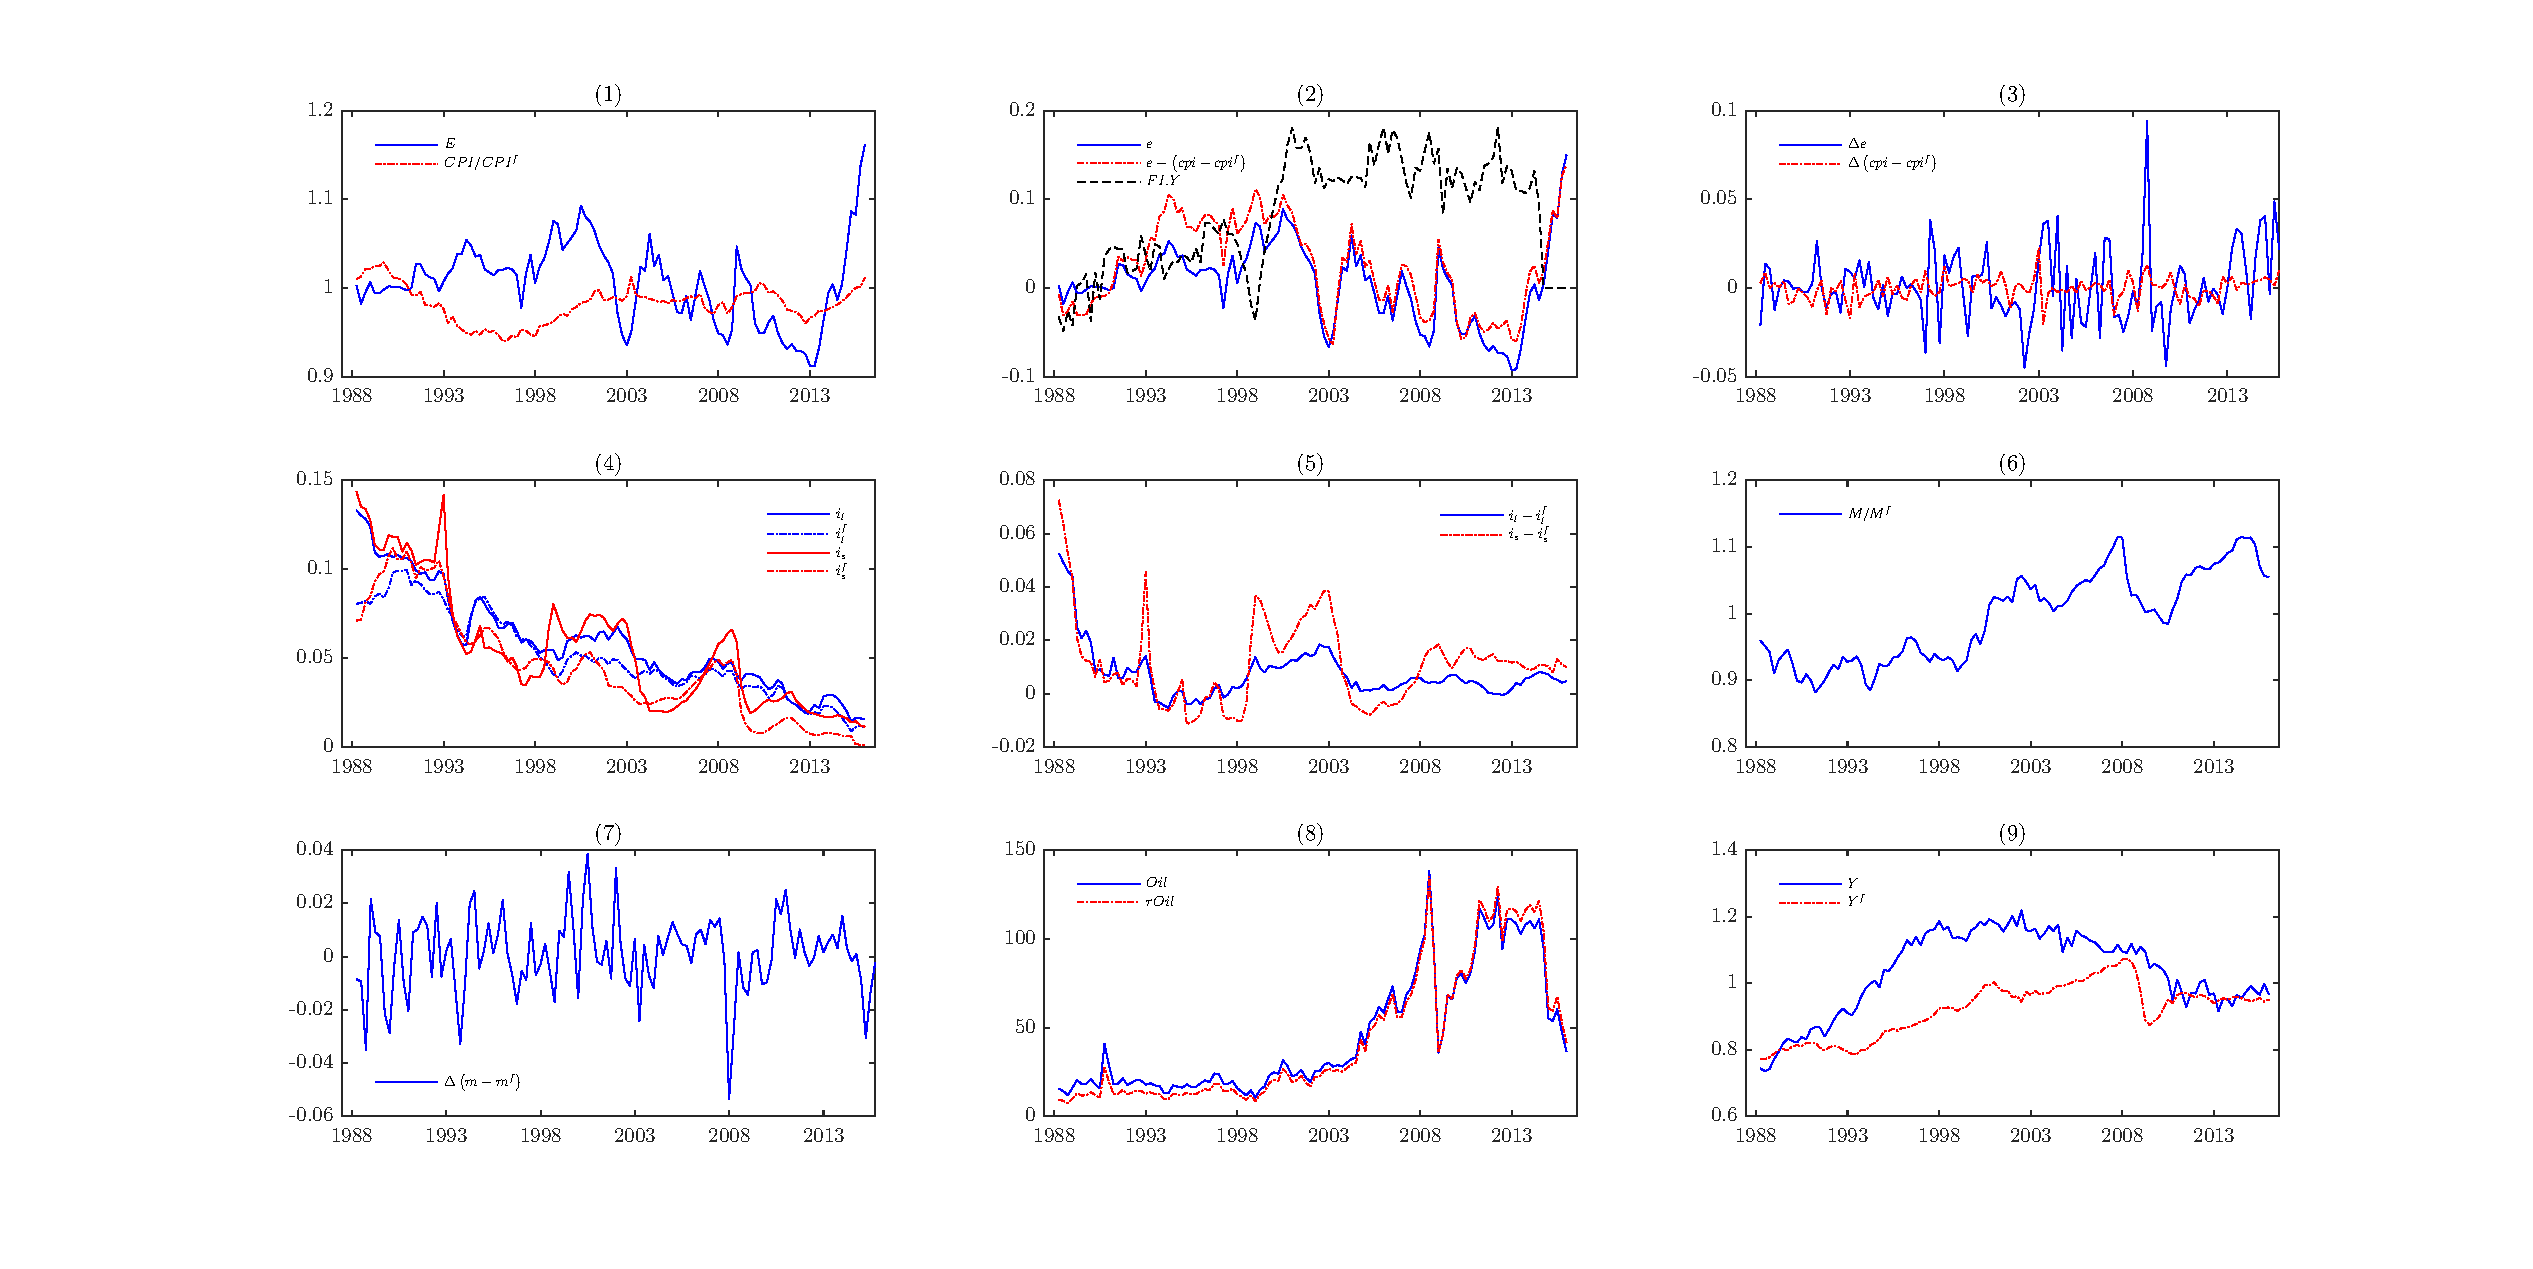
\includegraphics[height=0.9\textwidth]{images/variables.eps}
\vspace*{-1,5cm}\caption{\textit{Quarterly observations of selected variables over the period 1988:1-2015:4. Lower case letters denote the natural logarithm of upper case letters.}}
\label{fig:tspvar}
\end{figure}
\end{landscape}

\global\pdfpageattr\expandafter{\the\pdfpageattr/Rotate -45}
\global\pdfpageattr\expandafter{\the\pdfpageattr/Rotate 0}

\newpage
\subsection{Test for Stationarity}
\label{subsec:station}

\small
\noindent A common problem with a standard Dickey-Fuller (DF) test is the assumption of no serial correlation in the residual term ($\epsilon_t$) of the tests AR(1) model, $ \Delta e_t = \mu + \left(\theta - 1 \right)e_{t-1} + \epsilon_t$. The null hypothesis given by $\theta = 1$ (non stationary series) would not suffice in the presence of serial correlated residuals, as the standard errors may lead to invalid inference. To counter for this, the AR(1) model is augmented (thereof the name) to an AR(p) model with a series of lagged first differences of the dependent variable.
\begin{align}
\Delta e_t = \mu + \left(\theta - 1 \right)e_{t-1} + \sum_{j=1}^p\Phi_j\Delta e_{t-j}+\epsilon_t
\label{eq:adfco}
\end{align}
\noindent where $p$ is the lag order. For series that have trend, the term $\delta T$ is added to \ref{eq:adfco}. The null hypothesis is unchanged ($\theta = 1$), but the serial correlation is no longer a problem due to the augmented term.

\scriptsize
\begin{tabularx}{\textwidth}{lrrrr}
\caption{\small ADF \citep{dickey1979distribution} test for unit root, AIC criterion\label{tab:adf}}\vspace*{-0,5cm}\\
    \parnoteclear\\
    \toprule
Series\parnote{Note: The p-values are in large brackets [.]. Dickey-Fuller critical values: (a) Constant without trend 5\% = -2.90, 1\% = -3.51, (b) constant with trend 5\% = -3.47, 1\% = -4.08. Sample: 1988:1-2008:4. Max lag order based on Schwert and AIC, see \cite{schwert2002tests}.} & \multicolumn{2}{c}{Constant without trend} & \multicolumn{2}{c}{Constant with trend} \\
      & \multicolumn{1}{c}{Levels} & \multicolumn{1}{c}{First differences} & \multicolumn{1}{c}{Levels} & \multicolumn{1}{c}{First differences} \\
      \midrule
$e$   & -3.442 [0.010] & -6.805 [0.000] & -3.430 [0.047] & -6.723 [0.000] \\
$cpi$ & -1.579 [0.489] & -9.686 [0.000] & -3.716 [0.027] & -9.773 [0.000] \\
$cpi^*$ & -0.554 [0.878] & -2.057 [0.263] & -2.333 [0.415] & -1.259 [0.897] \\
$cpi-cpi^*$ & -3.047 [0.031] & -1.914 [0.326] & -3.435 [0.047] & -2.271 [0.450] \\
$e-cpi+cpi^*$ & -2.298 [0.175] & -7.486 [0.000] & -2.381 [0.386] & -7.430 [0.000] \\
$i_l$ & -2.136 [0.231] & -6.628 [0.000] & -3.535 [0.036] & -5.743 [0.000] \\
$i_l^*$ & -0.995 [0.757] & -5.602 [0.000] & -3.309 [0.065] & -5.566 [0.000] \\
$i_s$ & -2.323 [0.165] & -6.330 [0.000] & -2.504 [0.326] & -6.358 [0.000] \\
$i_s^*$ & -1.224 [0.667] & -5.143 [0.000] & -1.227 [0.904] & -5.182 [0.000] \\
$i_l - i_l^*$ & -1.933 [0.317] & -2.125 [0.235] & -1.920 [0.644] & -2.137 [0.524] \\
$i_s - i_s^*$ & -3.504 [0.008] & -7.906 [0.000] & -3.469 [0.043] & -7.857 [0.000] \\
$i_{l,t-1}-\Delta cpi_{t-2}$ & -1.768 [0.397] & -7.749 [0.000] & -4.825 [0.001] & -7.774 [0.000] \\
$i_{s,t-1}-\Delta cpi_{t-2}$ & -2.430 [0.137] & -10.030 [0.000] & -2.589 [0.287] & -4.213 [0.004] \\
$m$   & 0.408 [0.983] & -5.600 [0.000] & -1.812 [0.699] & -5.622 [0.000] \\
$m^*$ & 1.792 [0.999] & -7.987 [0.000] & 0.503 [0.999] & -6.464 [0.000] \\
$m-m^*$ & -1.526 [0.521] & -6.798 [0.000] & -2.811 [0.193] & -6.753 [0.000] \\
$y$   & -2.157 [0.223] & -2.329 [0.163] & -0.653 [0.976] & -7.441 [0.000] \\
$y^*$ & -1.462 [0.553] & -2.714 [0.072] & -1.536 [0.817] & -2.719 [0.229] \\
$y-y^*$ & -1.717 [0.423] & -2.741 [0.067] & -1.793 [0.709] & -5.216 [0.000] \\
$FI.Y$ & -11.060 [0.000] & -11.770 [0.000] & -11.014 [0.000] & -11.692 [0.000] \\
$oil$ & -1.874 [0.343] & -8.614 [0.000] & -2.777 [0.210] & -8.535 [0.000] \\
$roil$ & -1.642 [0.457] & -8.594 [0.000] & -2.803 [0.201] & -8.515 [0.000] \\
\midrule
\end{tabularx}
\vspace*{-0,6cm}\parnotes

\newpage
\subsection{Test for Cointegration}
\label{subsec:coint}
\small
\noindent The \cite{engle1987co} test for cointegration uses two steps to test if a cointegration vector exists. This is done by investigating an estimated residual term ($\hat{\epsilon}$) for stationarity. By using ordinary least square, $\hat{\epsilon} = e_t - \hat{\mu} - \sum_{i=1}^n\hat{\beta_i}f_t$ is estimated. Applying the ADF test (see subsection \ref{subsec:station}) on ($\hat{\epsilon}$) checks for the presence of one (estimated) cointegrating relationship.\\
\indent To allow for more than one cointegrating relationship, the \cite{johansen1991estimation} test is used. The test is considered to be a multivariate generalization of the ADF test. The strategy and estimation - maximum likelihood - makes it possible to estimate the number of cointegrating vectors, with the assumption that one has more than two variables. There are two types of this test, either with trace or eigenvalues ($\lambda$). Both tests start out with the following VAR(p) model.
\begin{align}
    \Delta e_t = \mu + \mathbf{\Pi}e_{t-1} + \sum_{j=1}^p\mathbf{\Pi}_j\Delta e_{t-j}+\epsilon_t
\end{align}
\noindent The rank of matrix $\mathbf{\Pi}$, i.e. rank($\mathbf{\Pi}$) is the number cointegrating vectors. If the variables are cointegrated then rank($\mathbf{\Pi}$) $\neq 0$. By the trace test, one tests the null hypothesis that the rank($\mathbf{\Pi}$) is $r_0$. The alternative hypothesis is that $r_0 < \text{rank}(\mathbf{\Pi}) \leq n$, where $n$ is the maximum possible cointegrating vectors. With the maximum eigenvalue test, the null hypothesis is that rank($\mathbf{\Pi}$) = 0 and the alternative, rank($\mathbf{\Pi}$) = 1.\\

\scriptsize
\begin{tabularx}{\textwidth}{lrrrr}
\caption{\small \cite{engle1987co} and \cite{johansen1991estimation} test for cointegration\label{tab:coint}}\vspace*{-0,5cm}\\
\parnoteclear\\
    \toprule
    \multicolumn{5}{c}{PANEL I: Engle-Granger two step procedure}\\
    \midrule
& \multicolumn{2}{c}{Constant without trend} & \multicolumn{2}{c}{Constant with trend}\\    
    \midrule
Series & $\left(\hat{\alpha} - 1  \right)$ & $\tau$-ADF & $\left(\hat{\alpha} - 1  \right)$ & $\tau$-ADF\\
    \midrule
& -0.238 & -3.169 [0.783] & -0.252 & -3.330 [0.823]\\
    \midrule
    \multicolumn{5}{c}{PANEL II: Johansen test}\\    
    \midrule
Series\parnote{Note: Unrestricted constant with common lag order of 4 ( = p). Variables tested: $e$, $e-cpi+cpi^*$, $i_s$, $i_s^*$ $m-m^*$, $y-y^*$ and $roil$. All of whom are I(1) at 1\% significance, see Table \ref{tab:adf}}      &       &       &       & Adj. for sample size \\
Rank  & Eigenvalue & Trace Test & $\lambda$-max Test & Trace Test \\
    \midrule    
0     & 0.642 & 205.37 [0.0000] & 82.211 [0.0000] & 205.37 [0.0000] \\
1     & 0.439 & 123.16 [0.0001] & 46.175 [0.0064] & 123.16 [0.0011] \\
2     & 0.317 & 76.989 [0.0107] & 30.496 [0.1204] & 76.989 [0.0277] \\
3     & 0.237 & 46.493 [0.0653] & 21.671 [0.2455] & 46.493 [0.1005] \\
4     & 0.186 & 24.822 [0.1732] & 16.464 [0.2068] & 24.822 [0.2032] \\
5     & 0.088 & 8.3583 [0.4352] & 7.3461 [0.4578] & 8.3583 [0.4538] \\
6     & 0.013 & 1.0123 [0.3144] & 1.0123 [0.3144] & 1.0123 [0.3271] \\
    \midrule
\end{tabularx}
\vspace*{-0,6cm}\parnotes

\newpage
\small 
\section{Econometric Output}
\label{sec:outp}
\noindent This section contains all the relevant econometric output as obtained from Gretl and PcGive. The models estimated are mentioned in section \ref{sec:meth}. All the diagnostics tests used in the procedure are commented in the notes below the tables. The scripts used are available from the author on request. 

\subsection{Relative Money Supply Proportionality EqCM}
\captionof{table}{\small The EqCM with linear proportionality between exchange rate and relative money.\label{tab:ecmtab1}}
\begin{gather}
\toprule \notag   
\end{gather}
\vspace*{-1.9cm}\begin{gather}
\begin{split}
&\Delta \widehat{e} = 
-\underset{(-3.919)}{0.023}
+\underset{(3.958)}{0.0005}\,\mbox{$T$}
-\underset{(-2.605)}{0.228}\,\mbox{$\Delta (m_t - m_t^*)$}
+\underset{(4.744)}{0.241}\,\mbox{$(e_{t-1} - m_{t-1} + m_{t-1})$}\\
& -\underset{(-4.483)}{0.464}\,\mbox{$e_{t-1}$}
-\underset{(-22.251)}{0.044}\,\mbox{$id97q1$}
-\underset{(-8.352)}{0.032}\,\mbox{$id02q2$}
-\underset{(-4.413)}{0.032}\,\mbox{$id08q2$}
 +\underset{(10.400)}{0.071}\,\mbox{$id08q4$}
\end{split}
 \notag \\
\textit{Sample}:1988:2-2008:4, \quad T = 83, \quad k = 8, \quad \textit{Method: OLS} \notag 
\end{gather}
\footnotesize
\vspace*{-1.5cm}\begin{tabularx}{\textwidth}{ll}
\parnoteclear\\
\multicolumn{2}{c}{\small \textbf{Diagnostics}\parnote{Note: The t-values are in brackets (.) below the estimators with the p-value in square brackets [.] beside the test statistics in the diagnostics list. All of which are calculated using the heteroskedasticity and autocorrelation consistent (HAC) standard errors. The goodness-to-fit reported is the adjusted $R^2$. $\bar{\text{\textit{VIF}}}$(J) is the average variance inflation factor. Less than 10 may imply no multicollinearity problem. \textit{AR} 1 - 4 F(4, 70) tests for autocorrelation in the residual up to four lags. \textit{ARCH} $\chi^2$(4) tests for autoregressive conditional heteroscedasticity (ARCH) up to order 4 \citep{engle1982autoregressive}. \textit{Het}.$\chi^2$ (k) is the \cite{koenker1982robust} robust variant of the \cite{breusch1979simple} test for heteroscedasticity. \textit{Het}.$\chi^2$ ($p-1$) tests for heteroscedasticity using only the squares of regressors \citep{white1980heteroskedasticity}. \textit{Normality}.$\chi^2$ (2) tests for normality of residuals, and is that of \cite{jarque1980efficient}. \textit{RESET} F(1, 73) tests for misspesification of model functional form including both squares and cubes of the fitted values, see \cite{ramsey1969tests}. \textit{Logs}.LM.$\chi^2$ and \textit{Squares}.LM.$\chi^2$ are non-linearity tests \citep{saikkonen1988lagrange}.}}\\
\midrule
$\hat{\sigma}$ &= 1.533\%\\
\textit{Log-lik} & = 233.759\\ 
$R^2$ &= 0.452\\
$\bar{\text{\textit{VIF}}}$(J) &= 3.202\\
\textit{AR} 1 - 4 F(4, 70) & = 0.445 [0.776] \\
\textit{ARCH} $\chi^2$(4)  & = 6.985 [0.137] \\
\textit{Het}.$\chi^2$ ($k$) & = 12.66 [0.124] \\
\textit{Het}.$\chi^2$ ($p-1$) & = 14.020 [0.299] \\
\textit{Normality}.$\chi^2$ & = 1.367 [0.505] \\
\textit{RESET} F(1, 73) & = 1.755 [0.180] \\
\textit{Logs}.LM.$\chi^2$ & = 0.100 [0.752] \\
\textit{Squares}.LM.$\chi^2$ & = 9.127 [0.058] \\
\end{tabularx}
\begin{center}
\vspace*{-0,7cm}\begin{tabularx}{\textwidth}{lrlr}
\midrule
Mean dependent var &  0.000519 & S.D. dependent var &  0.020704 \\
Sum squared resid &  0.017391 & S.E. of regression &  0.015330 \\
$R^2$ &  0.505211 & Adjusted $R^2$ &  0.451720 \\
Log-likelihood &  233.7593 & Akaike criterion & $-$449.5186 \\
Schwarz criterion & $-$427.7491 & Hannan--Quinn & $-$440.7728 \\
$\hat{\rho}$ &  0.042501 & Durbin--Watson &  1.909118\\
\end{tabularx}
\end{center}
\vspace*{-1.3cm}\begin{gather}
\midrule \notag   
\end{gather}
\vspace*{-1.5cm}\parnotes

\newpage
\small
\subsection{Combined PPP and UIRP EqCM}
\captionof{table}{\small The EqCM with combined linear proportionality between PPP and UIRP.\label{tab:ecmtab2}}
\begin{gather}
\toprule \notag   
\end{gather}
\vspace*{-1.9cm}%%% the following needs the amsmath LaTeX package
\begin{gather}
\begin{split}
\Delta \widehat{e} = 
\underset{(0.672)}{0.005}&
-\underset{(-0.231)}{0.073}\,\mbox{$\Delta cpi_t$}
+\underset{(1.188)}{0.348}\,\mbox{$\Delta cpi_{t-1}$}
+\underset{(2.334)}{0.695}\,\mbox{$\Delta cpi_{t-2}$}
 -\underset{(-1.576)}{0.616}\,\mbox{$\Delta cpi_{t}^*$}\\
-\underset{(-0.919)}{0.249}\,\mbox{$\Delta cpi_{t-1}^*$}&
-\underset{(-2.158)}{0.859}\,\mbox{$\Delta i_{s,t}^*$}
-\underset{(-1.891)}{0.096}\,\mbox{($e_{t-1} - cpi_{t-1} + cpi_{t-1}$)}
 -\underset{(-0.900)}{0.125}\,\mbox{($i_{s,t-1} - i_{s,t-1}^*$)}\\
&-\underset{(-9.436)}{0.037}\,\mbox{$id97q1$}
-\underset{(-10.689)}{0.043}\,\mbox{$id02q2$}
-\underset{(-6.736)}{0.023}\,\mbox{$id08q2$}
+\underset{(9.920)}{0.076}\,\mbox{$id08q4$}
\end{split}
 \notag \\
\textit{Sample}:1988:4-2008:4, \quad T = 81, \quad k = 12, \quad \textit{Method: OLS} \notag
\end{gather}
\footnotesize
\vspace*{-1.5cm}\begin{tabularx}{\textwidth}{ll}
\parnoteclear\\
\multicolumn{2}{c}{\small \textbf{Diagnostics}\parnote{Note: The model is estimated by OLS, see Table \ref{tab:ecmtab1} for further information. {Logs}.LM.$\chi^2$ cannot be applied as all the variables are in log-form. Previously, the time trend (T) was included to conduct the test.}}\\
\midrule
$\hat{\sigma}$ &= 1.644\%\\
\textit{Log-lik} & = 224.894\\ 
$R^2$ &= 0.373\\
$\bar{\text{\textit{VIF}}}$(J) &= 1.255\\
\textit{AR} 1 - 4 F(4. 70) &= 0.143 [0.965] \\
\textit{ARCH} $\chi^2$(4)  &= 4.677 [0.322] \\
\textit{Het}.$\chi^2$ ($k$) &= 7.491 [0.824] \\
\textit{Het}.$\chi^2$ ($p-1$) &= 11.964 [0.917] \\
\textit{Normality}.$\chi^2$ &= 0.290 [0.865] \\
\textit{RESET} F(1. 73) &= 1.300 [0.279] \\
\textit{Logs}.LM.$\chi^2$ &= - \\
\textit{Squares}.LM.$\chi^2$  &= 9.375 [0.312] \\
\end{tabularx}
\begin{center}
\vspace*{-0,7cm}\begin{tabularx}{\textwidth}{lrlr}
\midrule
Mean dependent var &  0.000622 & S.D. dependent var &  0.020769 \\
Sum squared resid &  0.018382 & S.E. of regression &  0.016442 \\
$R^2$ &  0.467280 & Adjusted $R^2$ &  0.373271 \\
Log-likelihood &  224.8937 & Akaike criterion & $-$423.7874 \\
Schwarz criterion & $-$392.6595 & Hannan--Quinn & $-$411.2985 \\
$\hat{\rho}$ &  0.039514 & Durbin--Watson &  1.920154 \\
\end{tabularx}
\end{center}
\vspace*{-1.3cm}\begin{gather}
\midrule \notag   
\end{gather}
\vspace*{-1.5cm}\parnotes

\newpage
\small
\subsection{Linear Oil Price Effects EqCM}
\captionof{table}{\small The EqCM with Linear Oil Price Effects.\label{tab:ecmtab3}}
\begin{gather}
\toprule \notag   
\end{gather}
\vspace*{-1.9cm}%%% the following needs the amsmath LaTeX package
\begin{gather}
\begin{split}
\Delta \widehat{e} &= 
\underset{(1.713)}{0.005}
-\underset{(-2.619)}{0.886}\,\mbox{$\Delta cpi^*$}
+\underset{(2.193)}{0.176}\,\mbox{$\Delta FI.Y_2$}
+\underset{(2.826)}{0.221}\,\mbox{$\Delta FI.Y_3$}
+\underset{(1.732)}{0.222}\,\mbox{$\Delta e_{t-2}$}\\
 +\underset{(2.354)}{0.198}\,\mbox{$\Delta e_{t-3}$}
 &-\underset{(-4.773)}{0.364}\,\mbox{$(e_{t-1} - roil_{t-1})$}
-\underset{(-12.819)}{0.042}\,\mbox{$id97q1$}
-\underset{(-15.807)}{0.039}\,\mbox{$id02q2$}
-\underset{(-3.399)}{0.012}\,\mbox{$id08q2$}\\
&+\underset{(11.850)}{0.071}\,\mbox{$id08q4$}
\end{split}
 \notag \\
\textit{Sample}:1989:1-2008:4, \quad T = 80, \quad k = 10, \quad \textit{Method: OLS} \notag
\end{gather}
\footnotesize
\vspace*{-1.5cm}\begin{tabularx}{\textwidth}{ll}
\parnoteclear\\
\multicolumn{2}{c}{\small \textbf{Diagnostics}\parnote{Note: The model is estimated by OLS, see Table \ref{tab:ecmtab1} for further information. {Logs}.LM.$\chi^2$ cannot be applied as all the variables are in log-form. Previously, the time trend (T) was included to conduct the test.}}\\
\midrule
$\hat{\sigma}$ &= 1,498\%\\
\textit{Log-lik} & = 228.464\\ 
$R^2$ &= 0.484\\
$\bar{\text{\textit{VIF}}}$(J) &= 1.203\\
\textit{AR} 1 - 4 F(4, 70) &= 1.018 [0.405] \\
\textit{ARCH} $\chi^2$(4)  &= 4.638 [0.326] \\
\textit{Het}.$\chi^2$ ($k$) &= 8.357 [0.594] \\
\textit{Het}.$\chi^2$ ($p-1$) &= 12.226 [0.728] \\
\textit{Normality}.$\chi^2$ &= 1.156 [0.561] \\
\textit{RESET} F(1, 73) &= 0.483 [0.619] \\
\textit{Logs}.LM.$\chi^2$ &= - \\
\textit{Squares}.LM.$\chi^2$  &= 4.152 [0.656] \\
\end{tabularx}
\begin{center}
\vspace*{-0,7cm}\begin{tabularx}{\textwidth}{lrlr}
\midrule
Mean dependent var &  0.000494 & S.D. dependent var &  0.020867 \\
Sum squared resid &  0.015492 & S.E. of regression &  0.014984 \\
$R^2$ &  0.549669 & Adjusted $R^2$ &  0.484404 \\
Log-likelihood &  228.4643 & Akaike criterion & $-$434.9286 \\
Schwarz criterion & $-$408.7263 & Hannan--Quinn & $-$424.4233 \\
$\hat{\rho}$ &  0.061376 & Durbin--Watson &  1.857504 \\
\end{tabularx}
\end{center}
\vspace*{-1.3cm}\begin{gather}
\midrule \notag   
\end{gather}
\vspace*{-1.5cm}\parnotes


\newpage

\small
\addcontentsline{toc}{section}{References}
\bibliographystyle{apalike} 
\bibliography{Master}
\end{spacing}


\includepdf[width=1.5\textwidth,height=1.45\textheight]{m-bakside_a4.pdf}

\end{document}